\documentclass[a4paper,14pt,oneside,openany]{article}


\usepackage{listings}
\usepackage{indentfirst} 

\usepackage{fontspec}     
\setmainfont{CMU Serif}   
\newfontfamily\cyrillicfonttt{DejaVu Sans Mono} 
\usepackage{polyglossia}
\setdefaultlanguage{russian}
\setotherlanguage{english}

\renewcommand{\lstlistingname}{Листинг}
% Отображение страницы
\usepackage{geometry} % размеры листа и отступов
\geometry{
	left=12mm,
	top=25mm,
	right=15mm,
	bottom=17mm,
	marginparsep=0mm,
	marginparwidth=0mm,
	headheight=10mm,
	headsep=7mm,
	nofoot}
\usepackage{afterpage,fancyhdr} % настройка колонтитулов
\pagestyle{fancy}
\fancypagestyle{style}{ % создание нового стиля style
	\fancyhf{} % очистка колонтитулов
	\fancyhead[LO, RE]{} % название документа наверху
	\fancyhead[RO, LE]{\leftmark} % название section наверху
	\fancyfoot[RO, LE]{\thepage} % номер страницы справа внизу на нечетных и слева внизу на четных
	\renewcommand{\headrulewidth}{0.25pt} % толщина линии сверху
	\renewcommand{\footrulewidth}{0pt} % толцина линии снизу
}
\fancypagestyle{plain}{ % создание нового стиля plain -- полностью пустого
	\fancyhf{}
	\renewcommand{\headrulewidth}{0pt}
}
\fancypagestyle{title}{ % создание нового стиля title -- для титульной страницы
	\fancyhf{}
	\fancyhead[C]{{\footnotesize \Large
			Министерство образования и науки Российской Федерации\\
			Федеральное государственное автономное образовательное учреждение высшего образования
	}}
	\fancyfoot[C]{{\large 
			Санкт-Петербург, \the\year
	}}
	\renewcommand{\headrulewidth}{0pt}
}

% Математика
\usepackage{amsmath, amsfonts, amssymb, amsthm} % Набор пакетов для математических текстов
%\usepackage{dmvnbase} % мехматовский пакет latex-сокращений
\usepackage{cancel} % зачеркивание для сокращений
% Рисунки и фигуры
\usepackage{graphicx}        
% \usepackage[unicode]{hyperref} % Was: \usepackage[unicode,pdftex]{hyperref}
\usepackage{wrapfig, subcaption} % вставка фигур, обтекая текст
\usepackage{caption} % для настройки подписей
\captionsetup{figurewithin=none,labelsep=period, font={small,it}} % настройка подписей к рисункам
% Рисование
\usepackage{tikz} % рисование
\usepackage{circuitikz}
\usepackage{pgfplots} % графики
% Таблицы
\usepackage{multirow} % объединение строк
\usepackage{multicol} % объединение столбцов
% Остальное
\usepackage{enumitem} % нормальное оформление списков
\usepackage{awesomebox}
\usepackage{tabularx}
\usepackage{hyperref} % гиперссылки
\usepackage{cleveref} % гиперссылки2

% Настройки стиля для листинга
\lstdefinestyle{mystyle}{
backgroundcolor=\color{gray!10!white},
basicstyle=\ttfamily,
language=Python,
numbers=left,
numberstyle=\small,
numbersep=5pt,
breaklines=true,
showstringspaces=false,
keywordstyle=\color{blue},
commentstyle=\color{green!40!black},
stringstyle=\color{green!40!black},
frame=single,
rulecolor=\color{black},
tabsize=2,
basicstyle=\small\ttfamily,
}


\setlist{itemsep=0.15cm,topsep=0.15cm,parsep=1pt} % настройки списков
% Теоремы, леммы, определения...
\theoremstyle{definition}
\newtheorem{Def}{Определение}
\newtheorem*{Axiom}{Аксиома}
\theoremstyle{plain}
\newtheorem{Th}{Теорема}
\newtheorem{Lem}{Лемма}
\newtheorem{Cor}{Следствие}
\newtheorem{Ex}{Пример}
\theoremstyle{remark}
\newtheorem*{Note}{Замечание}
\newtheorem*{Solution}{Решение}
\newtheorem*{Proof}{Доказательство}

\DeclareMathOperator{\sinc}{sinc}
\DeclareMathOperator{\Si}{Si}

% Свои команды
\newcommand{\comb}[1]{\left[\hspace{-4pt}\begin{array}{l}#1\end{array}\right.\hspace{-5pt} } % совокупность уравнений
% Титульный лист
\usepackage{csvsimple-l3}


\newcommand\tab[1][1cm]{\hspace*{#1}}

% https://tex.stackexchange.com/questions/2705/typesetting-column-vector
% Column Vector Macros
% EXAMPLE: \colvec{5}{a}{b}{c}{d}{e}
\newcount\colveccount
\newcommand*\colvec[1]{
        \global\colveccount#1
        \begin{pmatrix}
        \colvecnext
}
\def\colvecnext#1{
        #1
        \global\advance\colveccount-1
        \ifnum\colveccount>0
                \\
                \expandafter\colvecnext
        \else
                \end{pmatrix}
        \fi
}

% https://tex.stackexchange.com/questions/39051/typesetting-a-row-vector
% Row Vector Macros
% EXAMPLE: \rowvec{a,b,c,d,e}
\newcommand*{\rowvec}[1]{\left( #1\right)}

% \ExplSyntaxOn
% \clist_new:N \l_feq_vector_clist
% \NewDocumentCommand{\feqvector}{O{\\}mO{b}}{
%   \clist_set:Nn \l_feq_vector_clist {#2} % Set the list
%   \begin{#3matrix}
%   \clist_use:Nn \l_feq_vector_clist {#1} % show it with separator from #1 (\\)
%   \end{#3matrix}
% }
% \ExplSyntaxOff

%%% Вставляем по очереди все содержательные части документа %%%
\thispagestyle{empty}

\begin{center}
    МИНИСТЕРСТВО НАУКИ И ВЫСШЕГО ОБРАЗОВАНИЯ \\ РОССИЙСКОЙ ФЕДЕРАЦИИ

    \vspace{20pt}

    Университет ИТМО

    \vspace{20pt}

    Факультет систем управления и робототехники
\end{center}

\vfill

\begin{center}
    ОТЧЁТ \\  
    по лабораторной работе  №4, вариант - 2 \\
    \textit{Линейные системы автоматического управления}

    \vspace{20pt}

    по теме: \\
    \uppercase{Точностные свойства системы, астатизмы и регуляторы}
\end{center}

\vfill

\noindent Студент: \\
\textit{Группа R3336 \hfill Поляков А.А.}


    \vspace{20pt}

    \noindent Предподаватель: \\
    \textit{к.т.н., доцент \hfill  Пашенко А.В.}

\vfill

\begin{center}
    Санкт-Петербург \\ 2024
\end{center}

\begin{document}
\titlePage                                          % Титульник
\pagestyle{style}
\newpage

\tableofcontents                                   % Автособираемое оглавление

\label{ch:chap1}

\section{Исследование управляемости}
 
\subsection{Условие задания}

Необходимо рассмотреть систему:
$$
  \dot{x} = Ax+Bu
$$

Рассмотреть математическую модель в форме дифференциального уравнения при коэффициентах 
$a_2 = 9, a_1 = 26, a_0 = 24, b_2 = 2, b_1 = 6$, $b _0 = 8$:

\begin{gather}
	\notag
	\dddot{y} + a_2\ddot{y} + a_1\dot{y} + a_0y = b_2\ddot{u} + b_1\dot{u} + b_0u\\
	% \label{eq:dy_init}
	\dddot{y} + 9\ddot{y} + 26\dot{y} + 24y = 2\ddot{u} + 6\dot{u} + 8u
\end{gather}

% На основании полученного дифференциального уравнения \eqref{eq:dy_init} с использованием блоков элементарных 
операций построить структурную схему одноканальной линейной динамической системы.

Выполнить моделирование при входном воздействии $u(t) = 1$ и нулевых начальных условиях 
$\ddot{y}(0)$, $\dot{y}(0)$, $y(0)$.

\subsection{Решение задания}

В нашем случае имеем следующие начальные данные:
\begin{equation}
A = \begin{pmatrix}
  1 & 1 & 1 \\
  1 & 1 & 1 \\
  1 & 1 & 1 
\end{pmatrix} \tab 
B = \rowvec{a,b,c,d,e}  \tab 
x_1 = \colvec{3}{1}{0}{0}
\end{equation}


\endinput
\chapter{Наблюдатель полного порядка}
\label{ch:chap2}
\section{Условие задачи}

Рассматреть систему:
$$
  \begin{cases}
    \dot{x} = Ax \\
    y = Cx
  \end{cases}
$$ и выполнить следующие шаги:

\begin{itemize}
    \item  Найти собственные числа матрицы $A$ и определить наблюдаемость каждого из них. 
    Сделать вывод об наблюдаемости и обнаруживаемости системы.
    \item  Построить схему моделирования системы с наблюдателем состояния $\dot{\hat{x}} = A\hat{x} + L(C\hat{x}-y  )$
    \item Для каждого из спектров:
    \begin{itemize}
        \item  Найти соответствующую матрицу коррекции наблюдателя $L$, обеспечивающую желаемый спектр.
        \item Определить собственные числа матрицы наблюдателя $(A+LC)$ и сравнить
        с желаемым спектром в подтверждение корректности синтеза наблюдателя.
        \item Выполнить компьютерное моделирование с начальными условиями системы 
        $x(0) = \begin{bmatrix} 1&1&1&1 \end{bmatrix}^T$ и наблюдателя $\hat{x}(0)=\begin{bmatrix}2 & 0& 0 &-1\end{bmatrix}^T $.
        Построить  сравнительные графики $x(t)$ и $\hat{x}(t)$, а также график ошибки наблюдателя
         $e(t) = x(t) - \hat{x}(t)$
    \end{itemize}
    \item Сопоставить полученные результаты компьютерного моделирования для рассмотренных спектров, 
    оценить возможные сравнительные преимущества и недостатки каждого из них.
\end{itemize}
    

\section{Решение задачи}

Параметры для объекта:
$$
  A = \begin{bmatrix}
    -40 & 16 & 9 & -7 \\
    -64 & 25 & 14 & -12 \\
    -26 & 11 & 7 & -3 \\
    48 & -18 & -14 & 8
  \end{bmatrix} \tab
  C = \begin{bmatrix}
    -7&-2&5&-3
  \end{bmatrix}
$$
И следующие спектры сходимости для синтеза наблюдателя:
$$
  \begin{aligned}
    \sigma_1 = \{-4,-4,-4,-4\} \\
    \sigma_2 = \{-4,-40,-400,-4000\} \\
    \sigma_3 = \{-4 \pm 5i, -4 \pm 6i\} 
  \end{aligned}
$$


\subsection{Исследование наблюдаемости системы}
Найдём собственные числа матрицы $A$:
$$
    \lambda_{1,2} = \pm 3i, \tab \lambda_{3,4} = \pm 2i,
$$
Можно заметить, что тут только комплексные моды, поэтому тип вектора состояния будет иметь колебательный характер.
Найдём матрицу наблюдаемости системы:
$$
V = \begin{bmatrix}
    C \\ CA \\ CA^2 \\ CA^3
\end{bmatrix} = \begin{bmatrix}
          -7     &     -2       &    5     &     -3 \\
        134      &   -53     &    -14       &   34 \\
          28    &     53   &     -110       &   12 \\
        -1076   &      347     &     56    &    -406

            \end{bmatrix}, \tab\rightarrow rank(V) = 4
$$

В таком случае по критерию Калмана - система полностью наблюдаема , а значит и все собственные числа наблюдаемы, и как следствие - система обнаруживаема.

Рассмотрим несколько вариантов синтеза наблюдателей, с разными спектрами:

\newpage
\begin{figure}[ht]
  \centering
  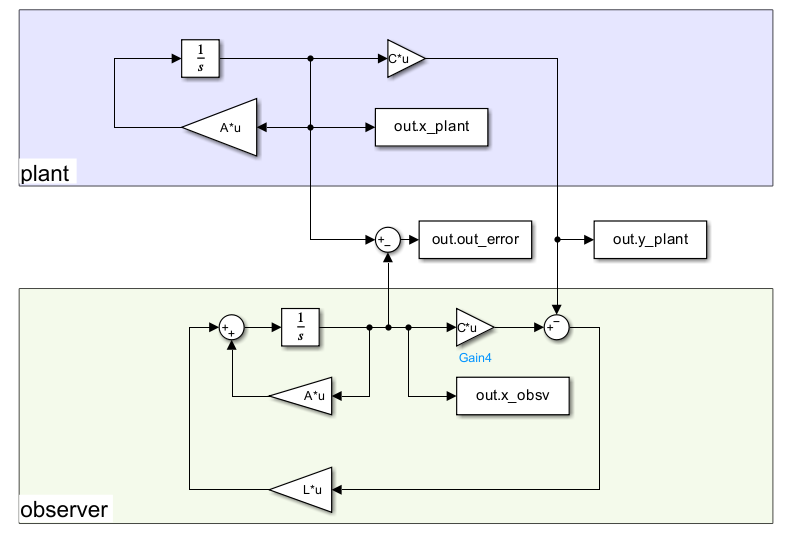
\includegraphics[width=0.8\textwidth]{model_observer.png}
  \caption{Модель с модальным наблюдателем}
\end{figure}

\subsection{Первый спектр}
$$
  \sigma_1 = \{-4,-4,-4,-4\}
$$
Система с наблюдателем полного порядка будет иметь следующие уравнения:
$$
\begin{cases}
  \dot{x} = Ax + Bu \\
  y = Cx 
\end{cases}, \tab 
\begin{cases}
  \dot{\hat{x}} = A\hat{x} + Bu +\mathbf{L}(\hat{y}-y)\\
  \hat{y} = C\hat{x} 
\end{cases}
$$

Для синтеза наблюдателя должны выполняться следующие условия:
$$
\begin{cases}
  \sigma(A)\cup\sigma(G)=\emptyset \\
  (G,Y) - \text{управляема, то всегда  существует } Q  \\
  (C,A) - \text{наблюдаема}
\end{cases}
$$
Тогда можно проследовать по алгоритму:
\begin{enumerate}
  \item Выбираем $G\in\mathbb{R}^{n\times n}$ с желаемым спектром $\sigma(G)$.
  \item Выбираем $Y\in\mathbb{R}^{n\times k}$ такую, чтобы пара $(G,Y)$ - была управляема.
  \item Найдем $Q\in\mathbb{R}^{n \times n}$ как решение уравнения Сильвестра $GQ - QA = YC$.
  \item Вычисляем матрицу коррекции наблюдателя: $L = Q^{-1}Y$
\end{enumerate}
Для получения $L$ возьмём следующую управляемую пару $G,Y$:
$$
G = \begin{bmatrix}
  -4  &   1  &   0  &   0 \\
  0  &  -4   &  1   &  0 \\
  0  &   0  &  -4  &   1 \\
  0   &  0   &  0  &  -4
\end{bmatrix}, \tab Y = \begin{bmatrix} 0\\1\\0\\1 \end{bmatrix},\tab \rightarrow \tab
L = \begin{bmatrix}
      11.08\\16.99\\9.74\\-15.62
    \end{bmatrix}
$$
Определим собственные числа матрицы наблюдателя $(A+LC)$:
$$
    \sigma_{obsv}=\{-4, -4, -4, -4 \}
$$
Однако я записал их в несколько округленном виде, поскольку мне не удалось подобрать удачный вектор $Y$, чтобы устранить такое отклонение:
$$
    \sigma_{true}=\{-4.0044, -4 + 0.0044i, -4 - 0.0044i, -3.9956 \}
$$
Но всё же погрежность здесь несколько незначительна, поэтому всё же сделаю вывод, что желаемые спектры совпали с спектром матрицы наблюдателя - синтез корректен.

Проведём моделирование, посмотрим на сравнительный график сходимости вектора состояния наблюдателя и системы, а также на их ошибку:
\newpage
\begin{figure}[ht]
  \centering
  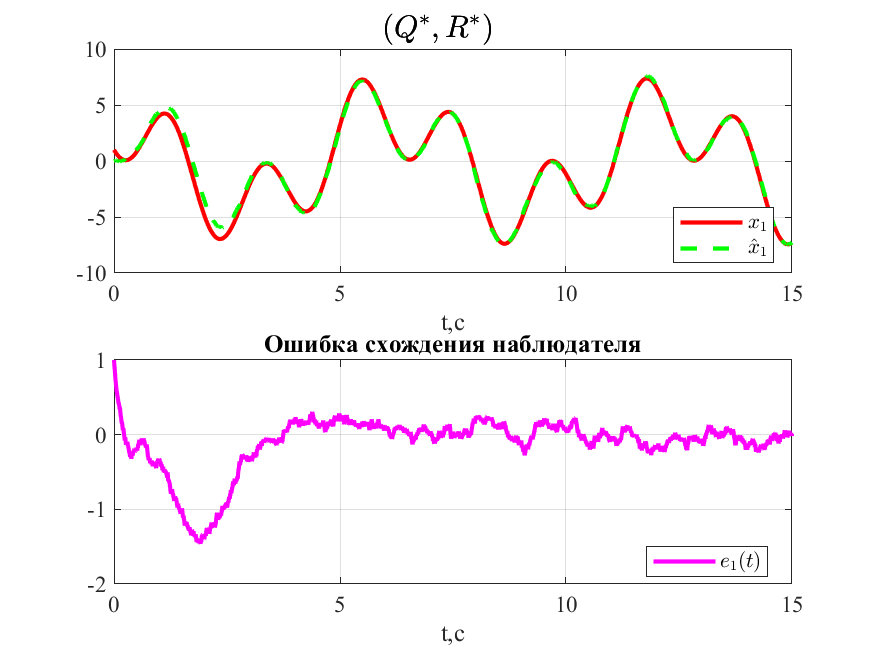
\includegraphics[width=0.8\textwidth]{obsv1.png}
  \caption{Состояние системы и ошибка сходимости}
\end{figure}
\begin{figure}[ht]
  \centering
  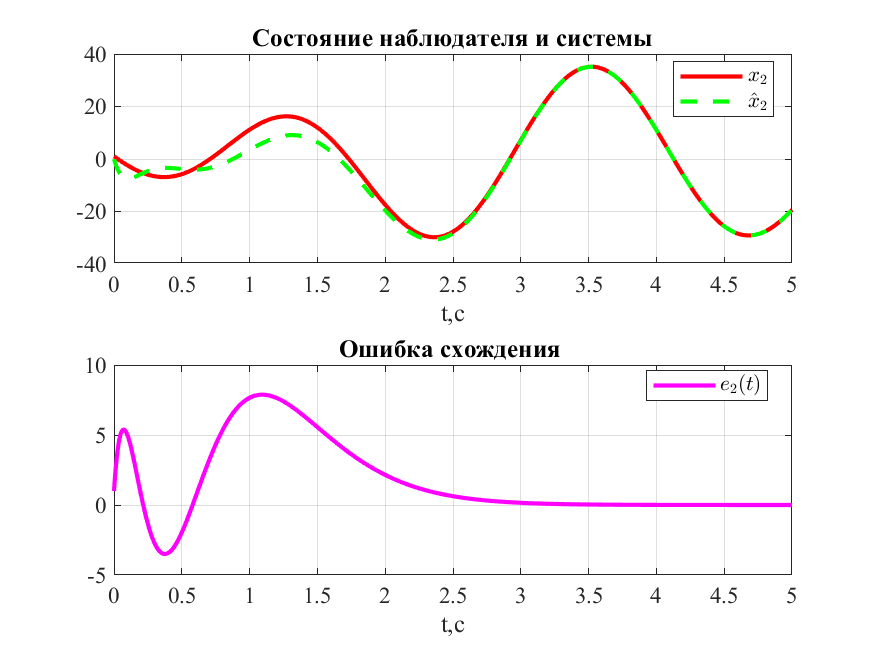
\includegraphics[width=0.8\textwidth]{obsv2.png}
  \caption{Состояние системы и ошибка сходимости}
\end{figure}
\newpage
\begin{figure}[ht]
  \centering
  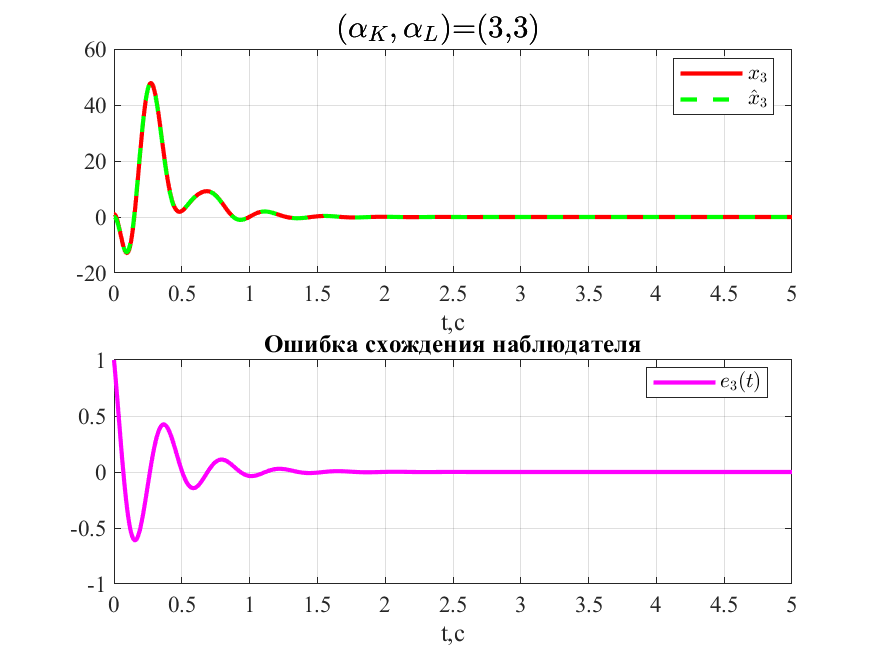
\includegraphics[width=0.8\textwidth]{obsv3.png}
  \caption{Состояние системы и ошибка сходимости}
\end{figure}
\begin{figure}[ht]
  \centering
  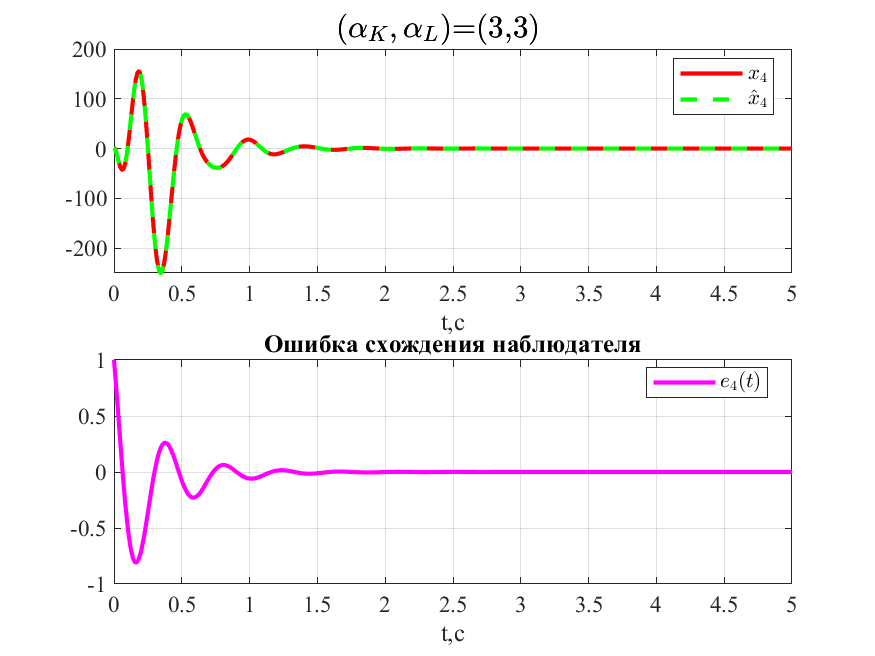
\includegraphics[width=0.8\textwidth]{obsv4.png}
  \caption{Состояние системы и ошибка сходимости}
\end{figure}


\newpage
\subsection{Второй спектр}
$$
  \sigma_2 = \{-4,-40,-400,-4000\}
$$

Для получения $L$ возьмём следующую управляемую пару $G,Y$:
$$
G = \begin{bmatrix}
  -4  &   0  &   0  &   0 \\
  0  &  -40   &  0   &  0 \\
  0  &   0  &  -400  &   0 \\
  0   &  0   &  0  &  -4000
\end{bmatrix}, \tab Y = \begin{bmatrix} 1\\1\\1\\1 \end{bmatrix},\tab \rightarrow \tab
L = 10^5\cdot\begin{bmatrix}
  3.157\\9.716\\12.754\\7.427
    \end{bmatrix}
$$
Определим собственные числа матрицы наблюдателя $(A+LC)$:
$$
    \sigma_{obsv}=\{-4, -40, -400, -4000 \}
$$
Можно сделать вывод, что желаемые спектры совпали с спектром матрицы наблюдателя - синтез корректен.
\begin{figure}[ht]
  \centering
  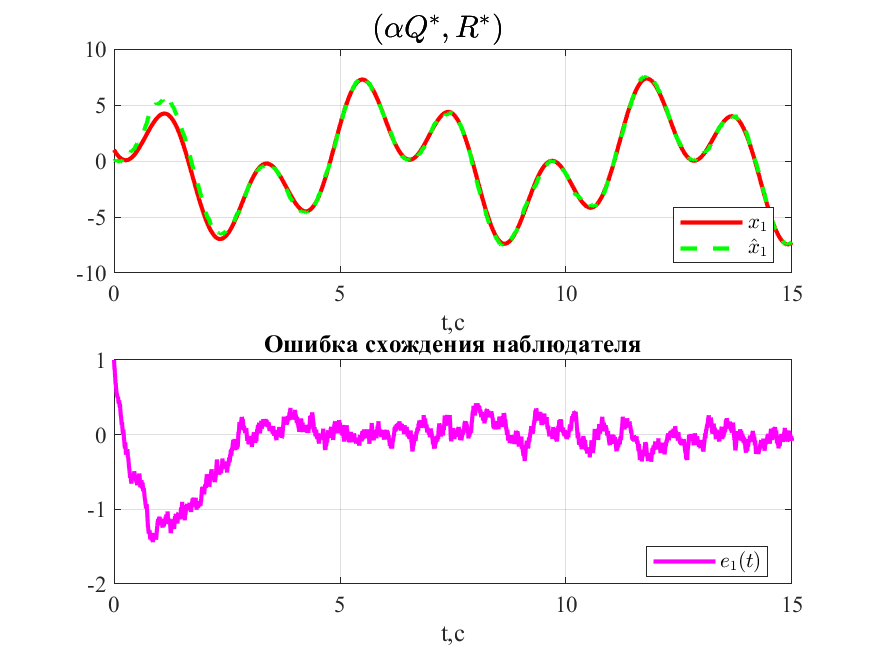
\includegraphics[width=0.8\textwidth]{obsv5.png}
  \caption{Состояние системы и ошибка сходимости}
\end{figure}
\newpage
\begin{figure}[ht]
  \centering
  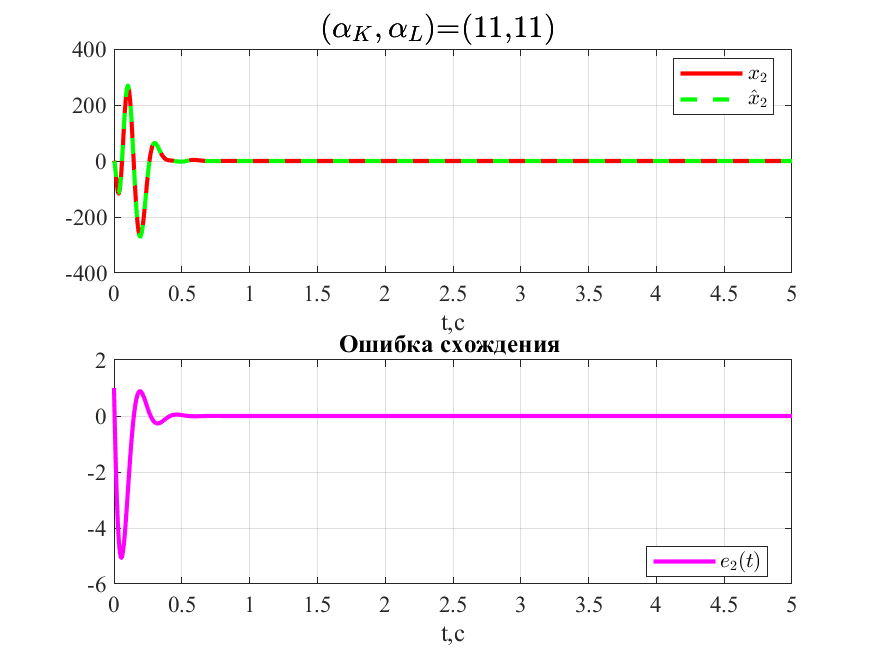
\includegraphics[width=0.8\textwidth]{obsv6.png}
  \caption{Состояние системы и ошибка сходимости}
\end{figure}
\begin{figure}[ht]
  \centering
  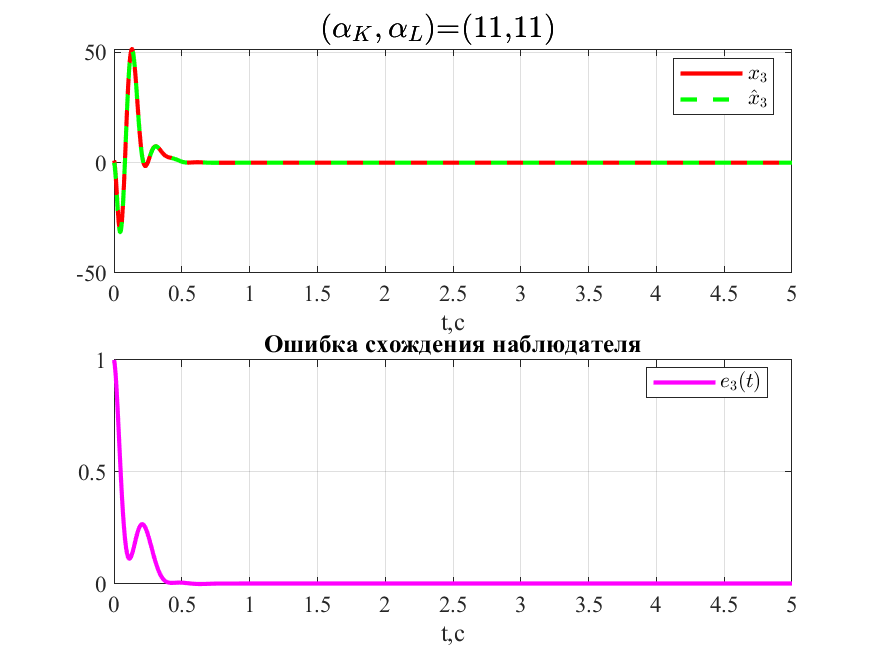
\includegraphics[width=0.8\textwidth]{obsv7.png}
  \caption{Состояние системы и ошибка сходимости}
\end{figure}
\newpage
\begin{figure}[ht]
  \centering
  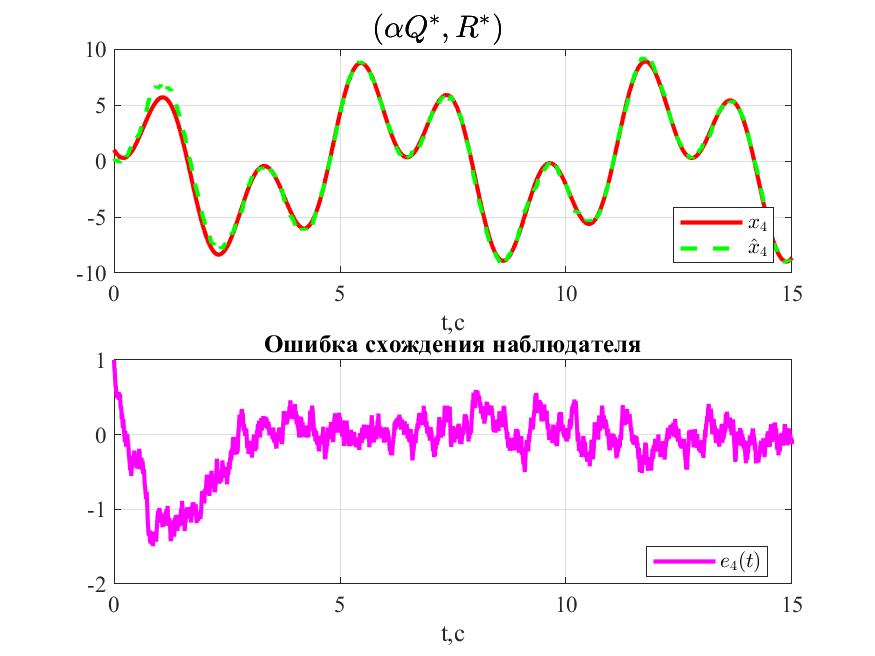
\includegraphics[width=0.8\textwidth]{obsv8.png}
  \caption{Состояние системы и ошибка сходимости}
\end{figure}


\newpage
\subsection{Третий спектр}
$$
  \sigma_3 = \{-4 \pm 5i, -4 \pm 6i\} 
$$

Для получения $L$ возьмём следующую управляемую пару $G,Y$:
$$
G = \begin{bmatrix}
  -4  &   5  &   0  &   0 \\
  -5  &  -4   &  0   &  0 \\
  0  &   0  &  -4  &   6 \\
  0   &  0   &  -6  &  -4
\end{bmatrix}, \tab Y = \begin{bmatrix} 0\\1\\0\\1 \end{bmatrix},\tab \rightarrow \tab
L = \begin{bmatrix}
  14.56\\25.87\\19.60\\-13.23
    \end{bmatrix}
$$
Определим собственные числа матрицы наблюдателя $(A+LC)$:
$$
    \sigma_{obsv}=\{-4 \pm 5i, -4 \pm 6i\}
$$
Можно сделать вывод, что желаемые спектры совпали с спектром матрицы наблюдателя - синтез корректен.
Проведём моделирование:
\begin{figure}[ht]
  \centering
  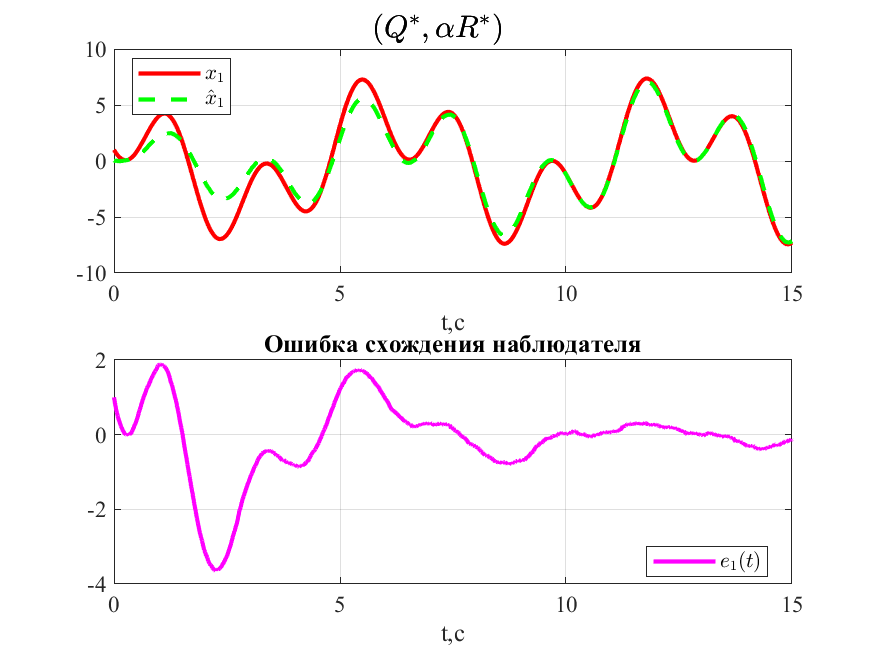
\includegraphics[width=0.8\textwidth]{obsv9.png}
  \caption{Состояние системы и ошибка сходимости}
\end{figure}
\newpage
\begin{figure}[ht]
  \centering
  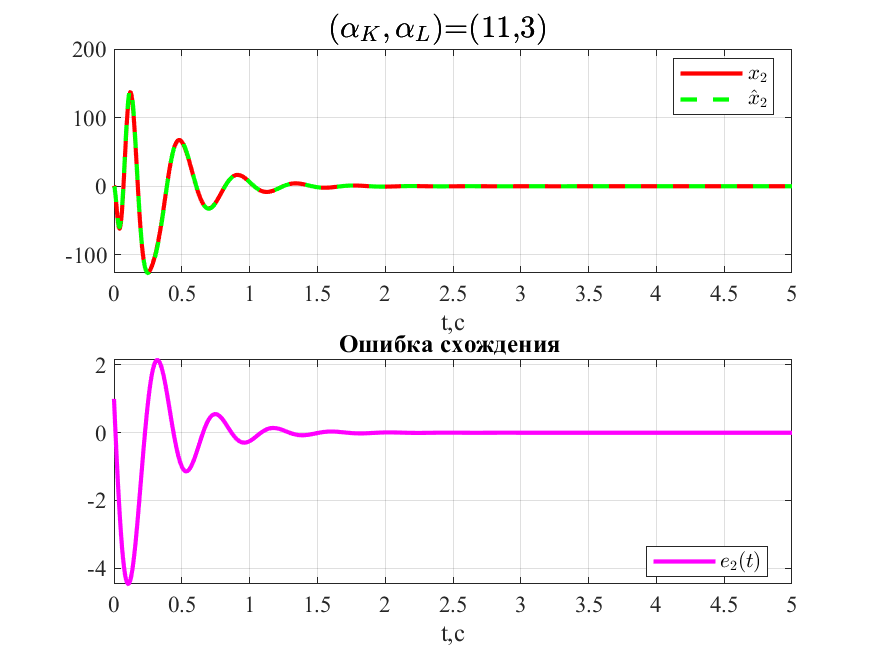
\includegraphics[width=0.8\textwidth]{obsv10.png}
  \caption{Состояние системы и ошибка сходимости}
\end{figure}
\begin{figure}[ht]
  \centering
  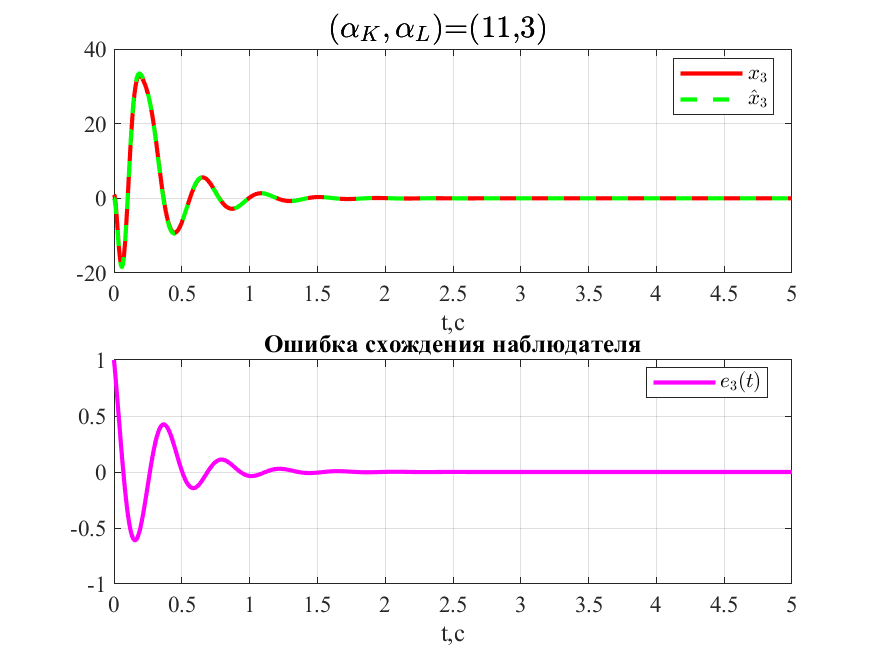
\includegraphics[width=0.8\textwidth]{obsv11.png}
  \caption{Состояние системы и ошибка сходимости}
\end{figure}
\newpage
\begin{figure}[ht]
  \centering
  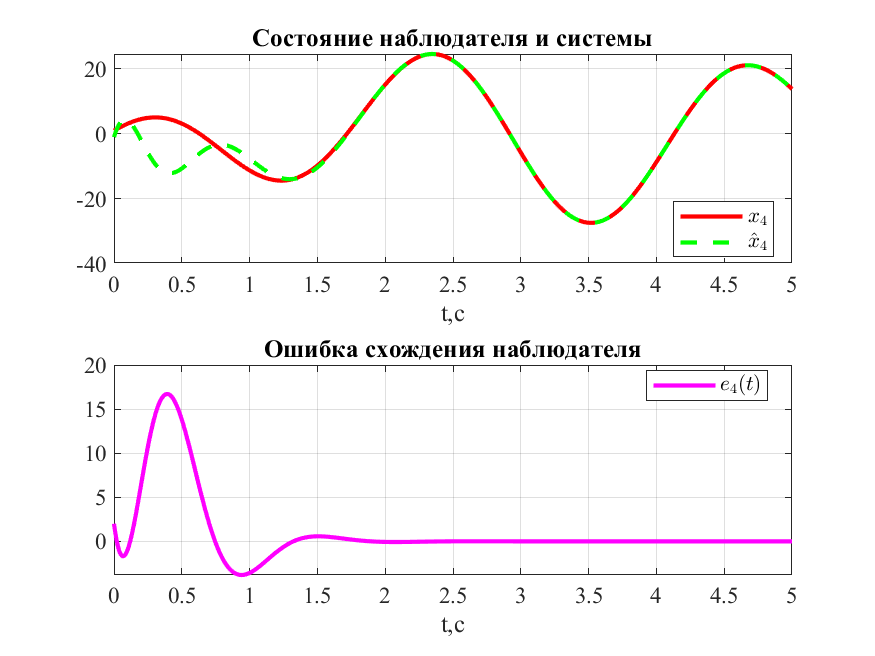
\includegraphics[width=0.8\textwidth]{obsv12.png}
  \caption{Состояние системы и ошибка сходимости}
\end{figure}


\newpage
\subsection{Сравнение выбора собственных чисел для синтеза наблюдателя}
Мы можем заметить, что происходят похожие процессы, как и при синтезе модального регулятора - выбор мод наблюдателя напрямую влияет на характер его схождения к истинной системе.
В первом случае спектр выбран не слишком большим, поэтому матрица коррекции не слишком велика, в итоге мы получили довольно большое перерегулирование (по графику ошибки) при небольшом времени переходного процесса.

Во втором случае мы получили довольно агрессивную сходимость(перерегулирования практически нет, время переходного процесса экстремально мало), но в реальных физических системах вряд ли
наша оценка может так быстро/резки сойтись к истинной безошибочно, 
потому что датчики шумные, и их фильтрация стоит какого-то времени на сбор достаточного количества данных, и последующуб обработку.

В третьем случае наш спектр состоял в том числе и из колебательных мод, поэтому переходный процесс был с перерегулированием куда больше, чем в первом случае, однако время этого процесса стало куда меньше.

\subsection{Вывод}
В этом задании мы работали с полностью наблюдаемой системой, это мы узнали через критерий Калмана.
Мы узнали, что синтезировать наблюдатели можно с разным "характером" сходимости. Для наблюдения мы 
синтезировали модального наблюдателя с помощью уравнения Сильвестра, а также провели серию моделирований с разными наблюдателями, все они показали то, 
что мы сходимся к оригинальной системе с разным качеством переходного процесса - его времени и перерегулирования.
\endinput 
\chapter{Запаздывание}
\label{ch:chap3}

В соответствии с моим вариантом:
$$
    j=2, \tab W_3(s) = \frac{7s+5}{s^2 + 4s}, \tab W_4(s) = \frac{20s^2 +1.6s +2}{10s^3-10s^2-0.1s+0.1}
$$
Необходимо добавить к каждой ПФ звено чистого запаздывания $e^{-\tau s}$.

\section{Передаточная функция $W_3$}

Рассмотрим обновлённую ПФ:
$$
    W_3(s) = \frac{7s+5}{s^2 + 4s}e^{-\tau s}
$$
Получаем её полюса: $\lambda_{1,2} = \{-4, 0\}$, система имеет два устойчивых полюса.

Построим для неё годографы, с разными $\tau$:
\begin{figure}[ht]
    \centering
    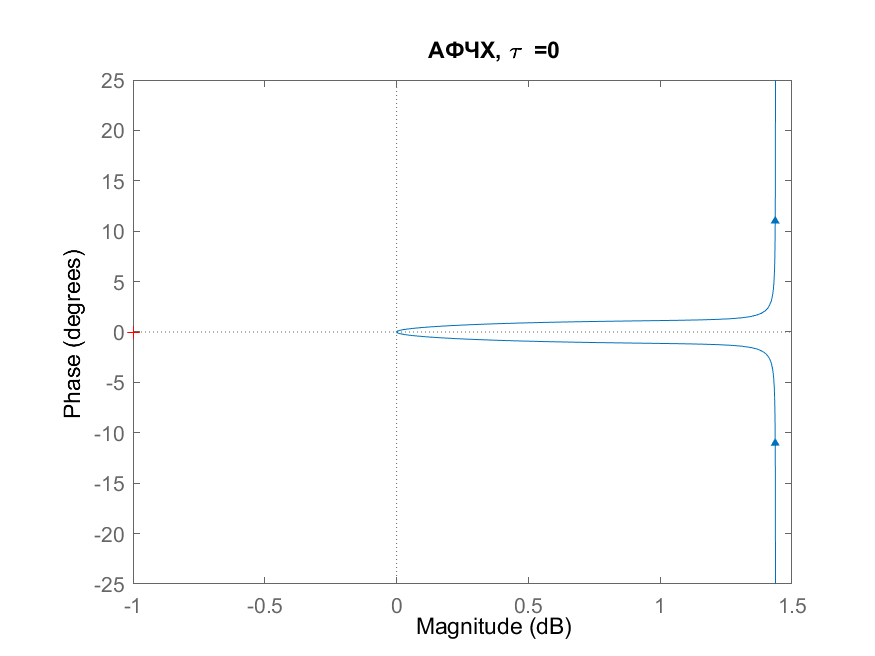
\includegraphics[width=0.7\textwidth]{nyquist_task31_object1.png}
    \caption{Годограф Найквиста для разомкнутой системы, $\tau=0$}
\end{figure}
\newpage
\begin{figure}[ht]
    \centering
    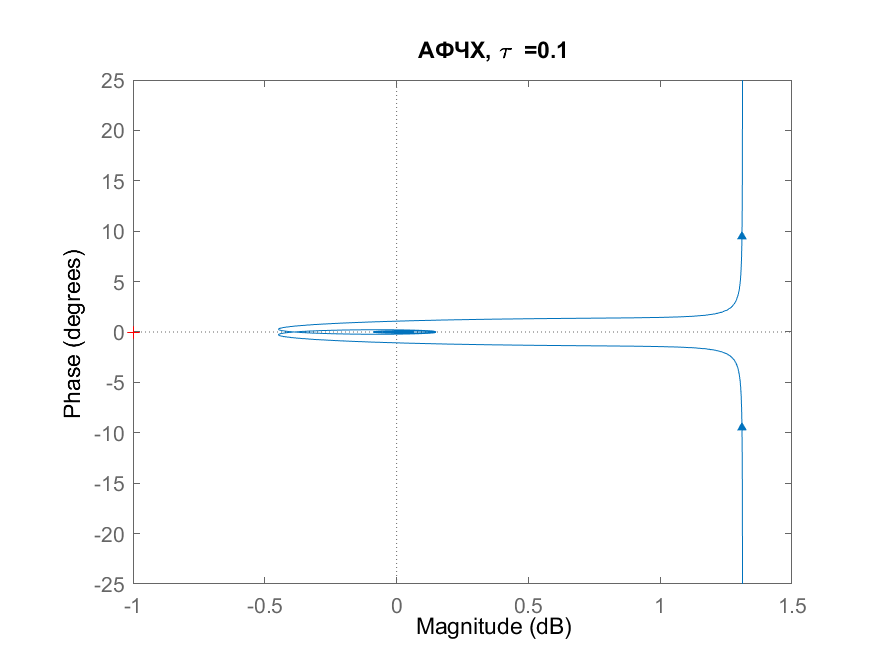
\includegraphics[width=0.7\textwidth]{nyquist_task32_object1.png}
    \caption{Годограф Найквиста для разомкнутой системы, $\tau=0.1$}
\end{figure}
\begin{figure}[ht]
    \centering
    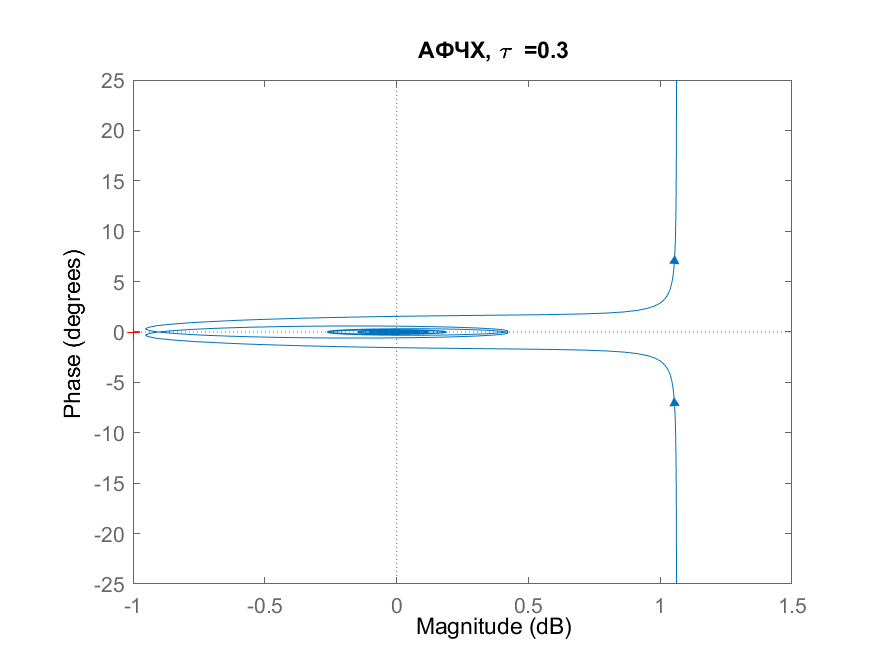
\includegraphics[width=0.7\textwidth]{nyquist_task33_object1.png}
    \caption{Годограф Найквиста для разомкнутой системы, $\tau=0.3$}
\end{figure}
\newpage
\begin{figure}[ht]
    \centering
    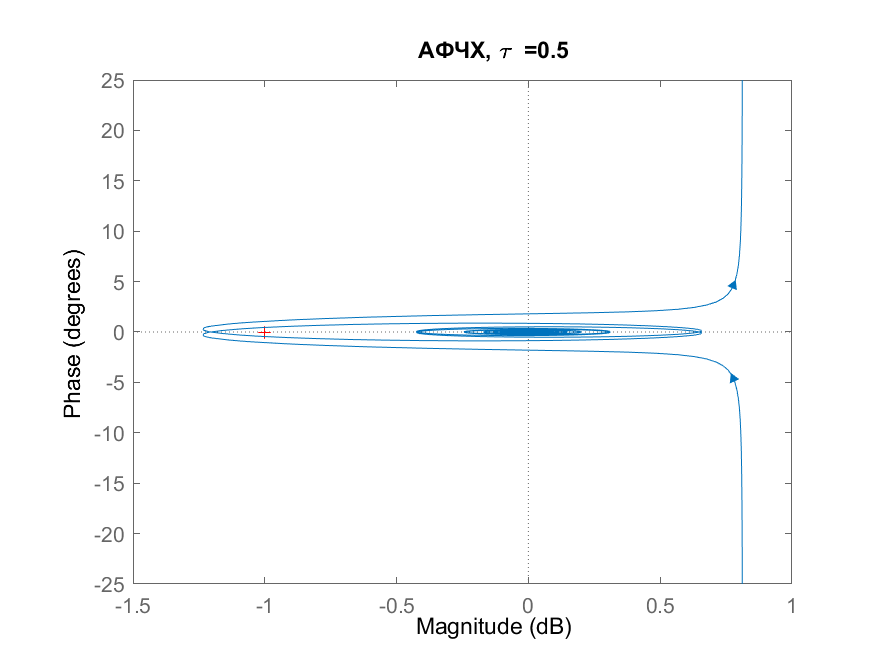
\includegraphics[width=0.7\textwidth]{nyquist_task34_object1.png}
    \caption{Годограф Найквиста для разомкнутой системы, $\tau=0.5$}
\end{figure}
\begin{figure}[ht]
    \centering
    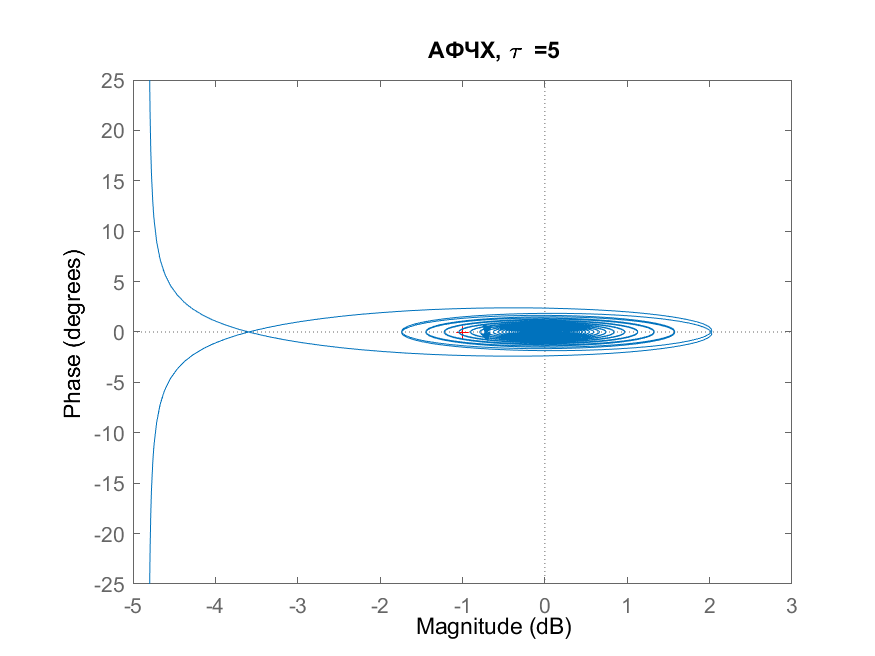
\includegraphics[width=0.7\textwidth]{nyquist_task35_object1.png}
    \caption{Годограф Найквиста для разомкнутой системы, $\tau=5$}
\end{figure}
\newpage
По полученным графикам можно заметить, что замкнутая система будет устойчива примерно до  $\tau< 0.4$, так как до $\tau < 0.3$ ещё всё хорошо и есть небольшой запас коэффицциента запаздывания. После же к системе прибавится два дополнительных неустойчивых полюсов, так как критическая точка попадёт внутрь годографа
и мы получим два оборота по часовой стрелке.

Давайте ниже узнаем точно диапазон - вычислим его аналитически\dots

\newpage
\subsection{Частотные характеристики}
Найдём критическое значение $\tau$. 

\begin{figure}[ht]
    \centering
    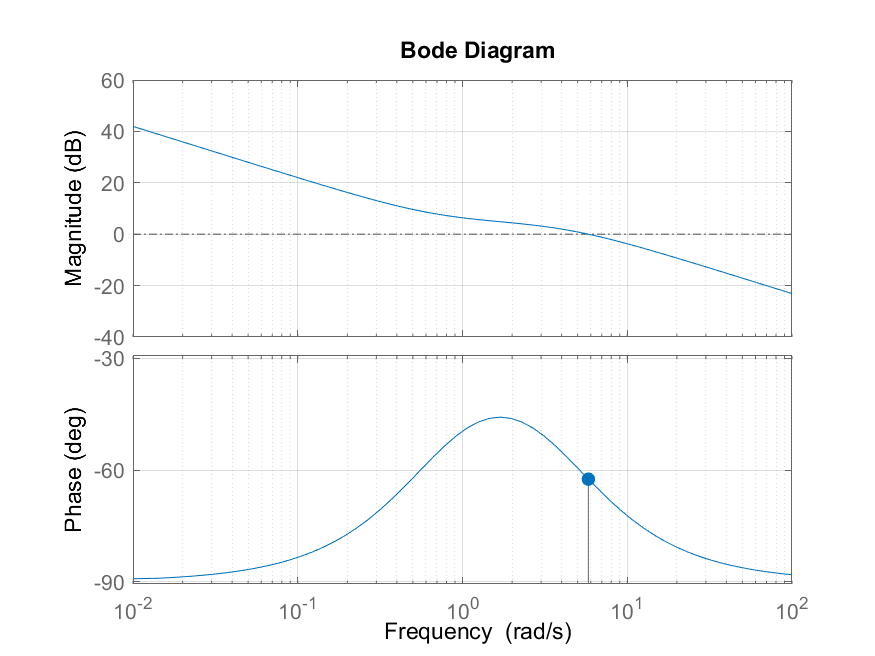
\includegraphics[width=0.7\textwidth]{log_nyquist_task3_object1.png}
    \caption{ЛАФЧХ, $\tau=5.0$}
\end{figure}
С помощью команды $\textrm{allmargin}$ получим информацию о критической точке на графике, её критическое значение и запас по фазе :
$$
 \tau_{crit} \approx 0.35, \tab \phi_3 \approx 117^\circ
$$

Теперь проверим аналитически, посчитаем $\tau_{crit}$, которые мы получили от \textit{matlab} до:
$$
\tau_{max} = \frac{\phi_3}{\omega_\phi}
$$, где $\phi_3$ - запас по фазе, $\omega_\phi$ - частота, соответствующая запасу по фазе. Эти два параметра мы можем найти для двух точек, если приблизим график достаточно точно, тогда получим:
$$
\tau_{crit} = \frac{117.54\pi}{180\cdot 5.8084} = 0.3537
$$

Как можно заметить, аналитически посчитанные совпали с ответами от \textit{allmargin}.


\newpage
\subsection{Переходные функции}
\begin{figure}[ht]
    \centering
    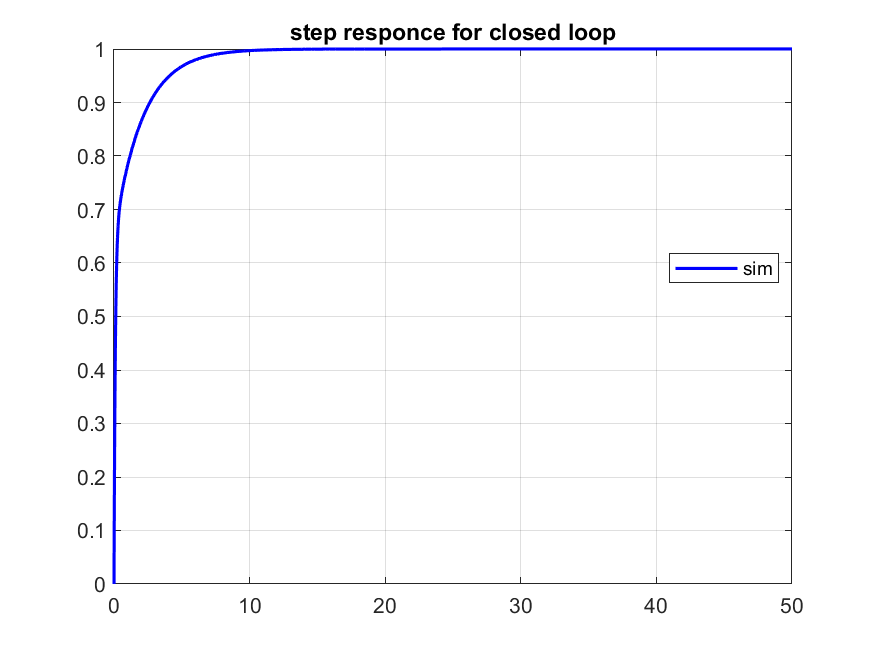
\includegraphics[width=0.7\textwidth]{step_responce31_closed1.png}
    \caption{Переходная функция для замкнутой системы, $\tau=0$}
\end{figure}
\begin{figure}[ht]
    \centering
    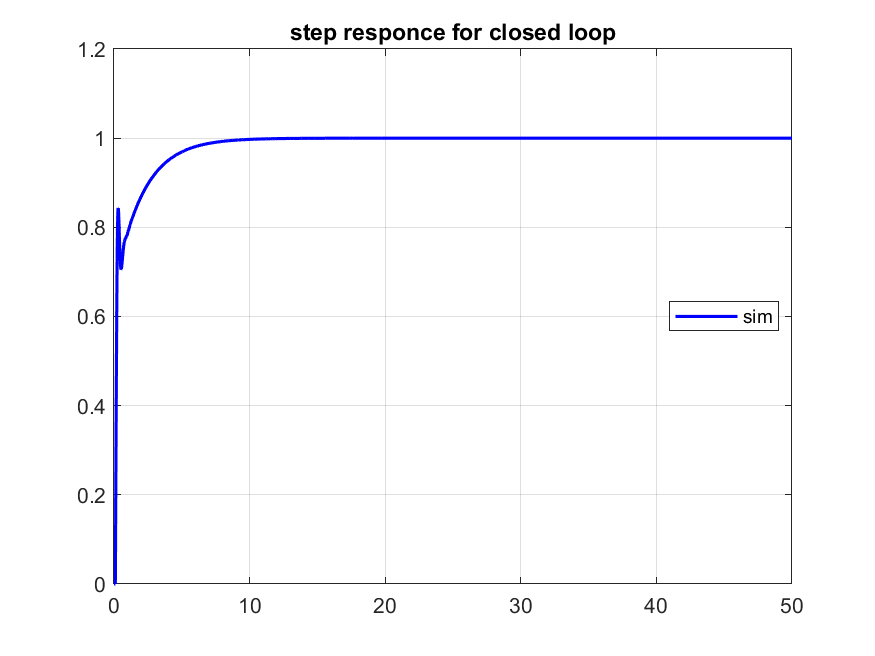
\includegraphics[width=0.7\textwidth]{step_responce32_closed1.png}
    \caption{Переходная функция для замкнутой системы, $\tau=0.1$}
\end{figure}

\newpage
\begin{figure}[ht]
    \centering
    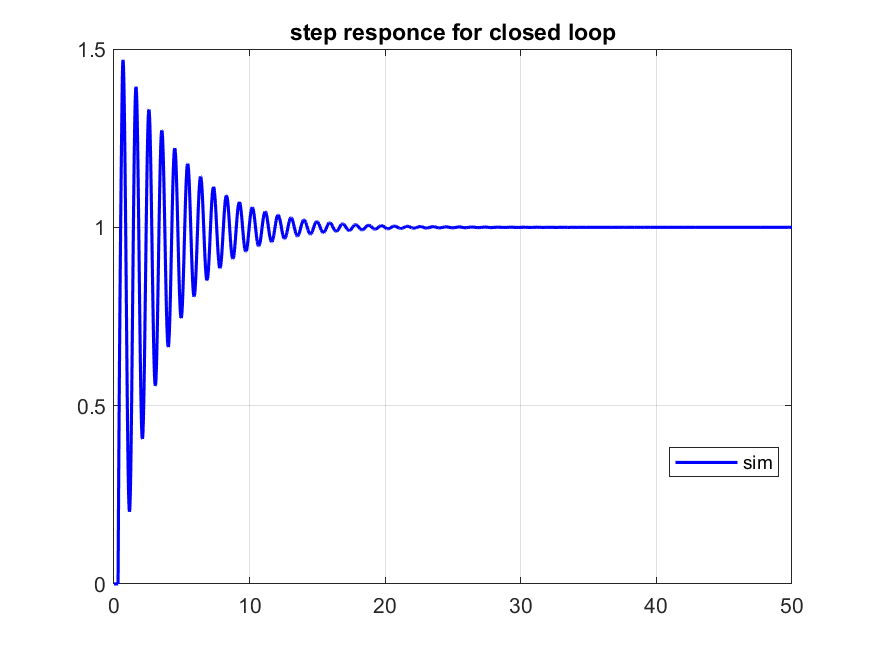
\includegraphics[width=0.7\textwidth]{step_responce33_closed1.png}
    \caption{Переходная функция для замкнутой системы, $\tau=0.3$}
\end{figure}
\begin{figure}[ht]
    \centering
    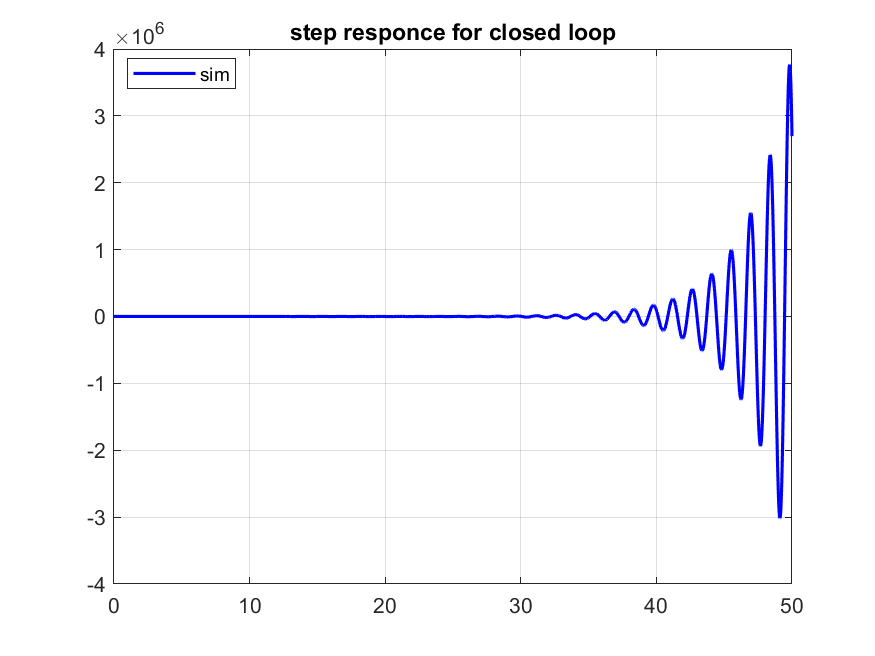
\includegraphics[width=0.7\textwidth]{step_responce34_closed1.png}
    \caption{Переходная функция для замкнутой системы, $\tau=0.5$}
\end{figure}
\newpage
\begin{figure}[ht]
    \centering
    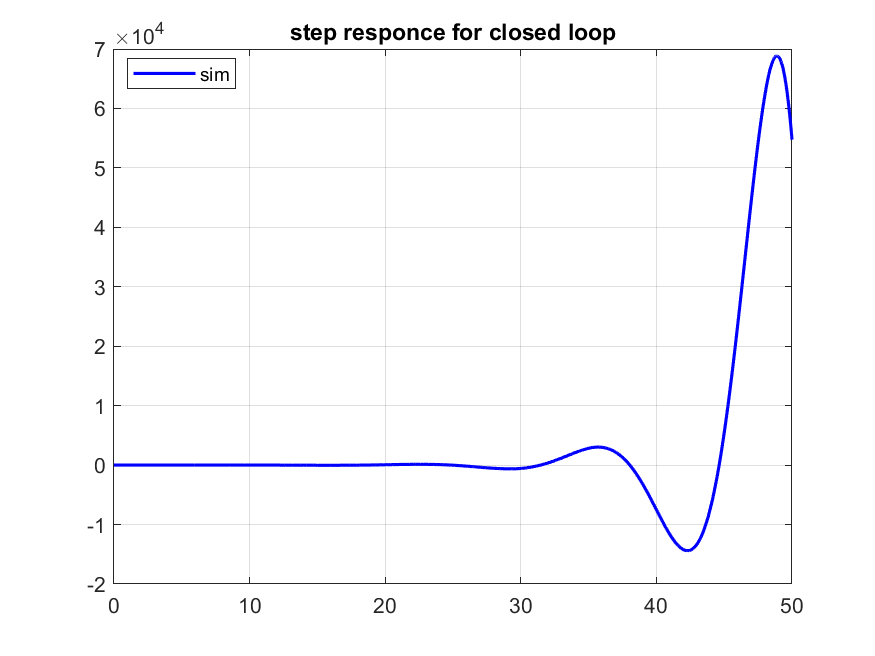
\includegraphics[width=0.7\textwidth]{step_responce35_closed1.png}
    \caption{Переходная функция для замкнутой системы, $\tau=5$}
\end{figure}
По графикам можно заметить, что аналитические выкладки подтвердились - замкнутая система устойчива будет устойчива лишь при $\tau < 0.35 $.


\section{Передаточная функция $W_4$}
Рассмотрим обновлённую ПФ:
$$
    W_4(s) = \frac{20s^2 +1.6s +2}{10s^3-10s^2-0.1s+0.1}e^{-\tau s}
$$
Получим её полюса: $\lambda_{1,2,3} \approx \{-0.23, 0.11 \pm 0.17j \}$, система имеет два неустойчивых и один устойчивых полюс.

Построим для неё годографы, с разными $\tau$:
\begin{figure}[ht]
    \centering
    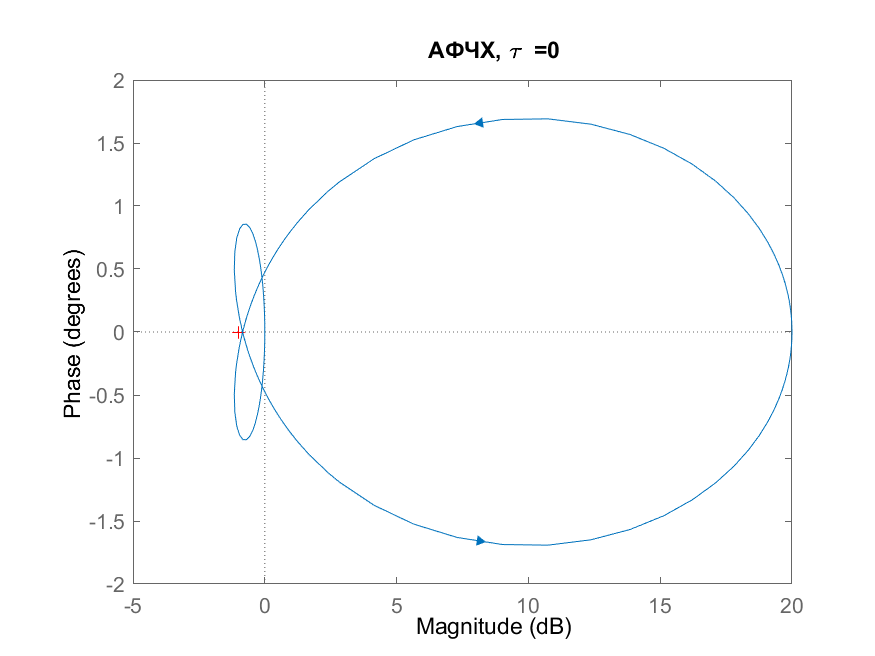
\includegraphics[width=0.7\textwidth]{nyquist_task31_object2.png}
    \caption{Годограф Найквиста для разомкнутой системы, $\tau=0$}
\end{figure}
\newpage
\begin{figure}[ht]
    \centering
    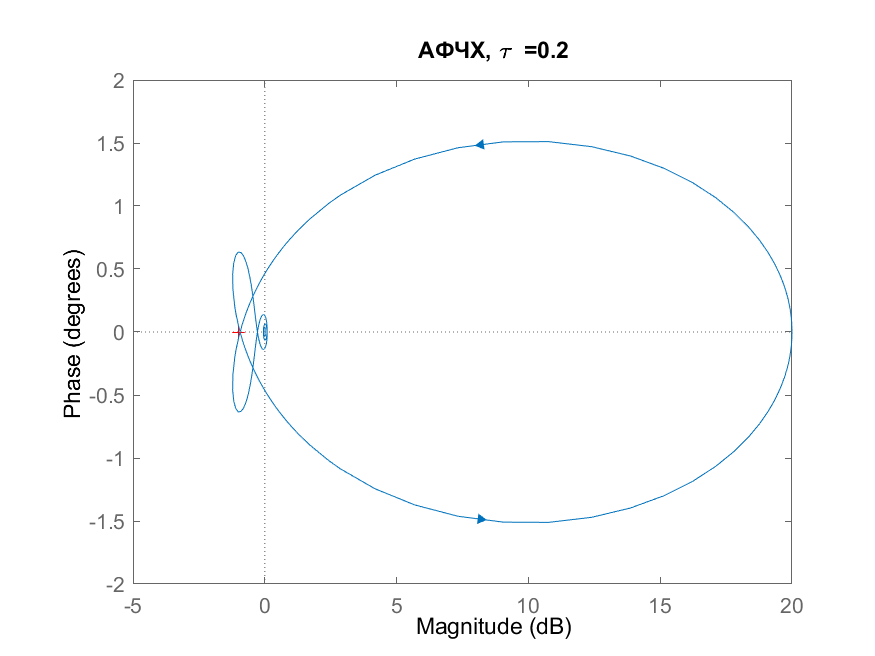
\includegraphics[width=0.7\textwidth]{nyquist_task33_object2.png}
    \caption{Годограф Найквиста для разомкнутой системы, $\tau=0.2$}
\end{figure}

\begin{figure}[ht]
    \centering
    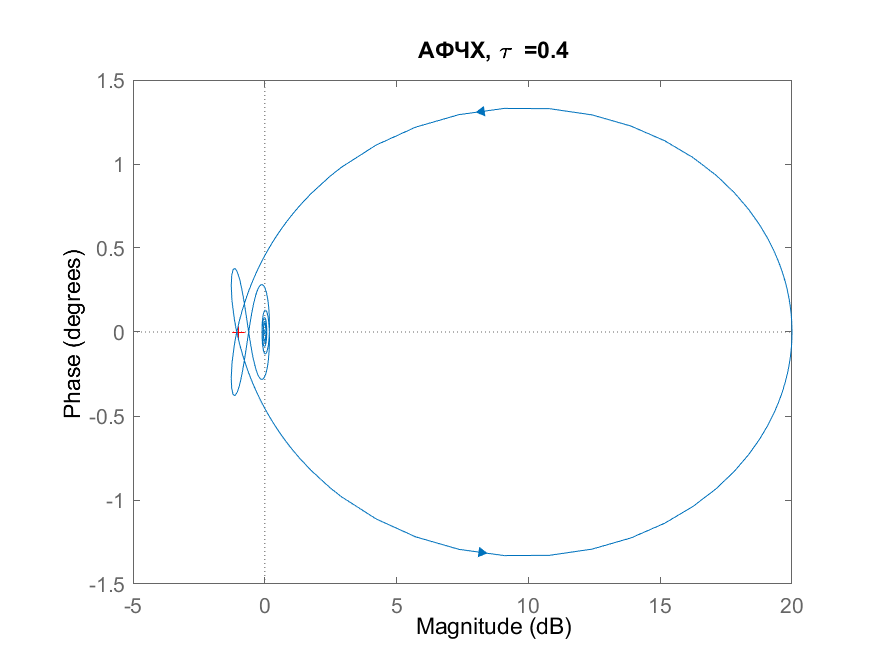
\includegraphics[width=0.7\textwidth]{nyquist_task35_object2.png}
    \caption{Годограф Найквиста для разомкнутой системы, $\tau=0.4$}
\end{figure}
\newpage
\begin{figure}[ht]
    \centering
    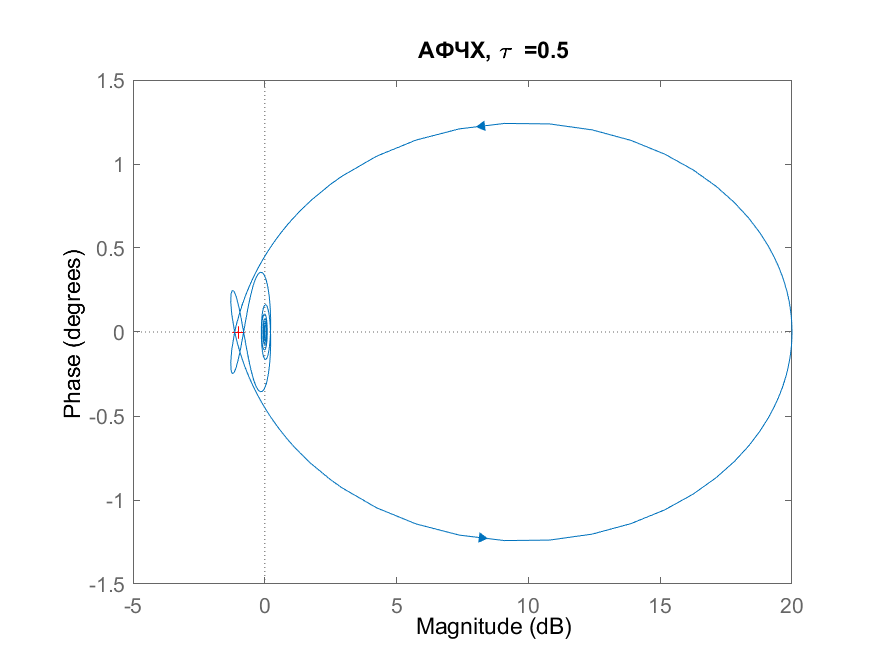
\includegraphics[width=0.7\textwidth]{nyquist_task36_object2.png}
    \caption{Годограф Найквиста для разомкнутой системы, $\tau=0.5$}
\end{figure}
\begin{figure}[ht]
    \centering
    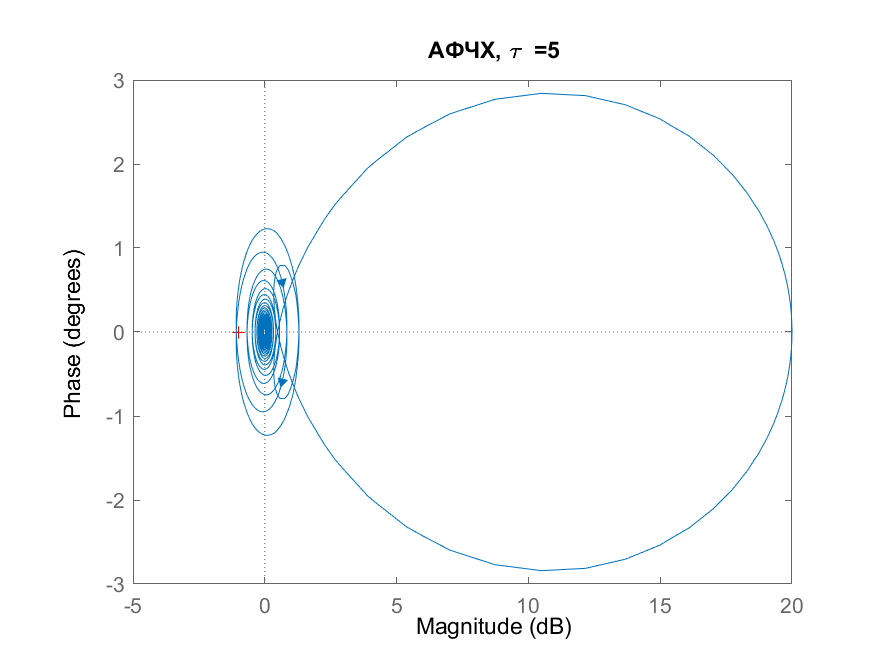
\includegraphics[width=0.7\textwidth]{nyquist_task39_object2.png}
    \caption{Годограф Найквиста для разомкнутой системы, $\tau=5$}
\end{figure}
\newpage
\begin{figure}[ht]
    \centering
    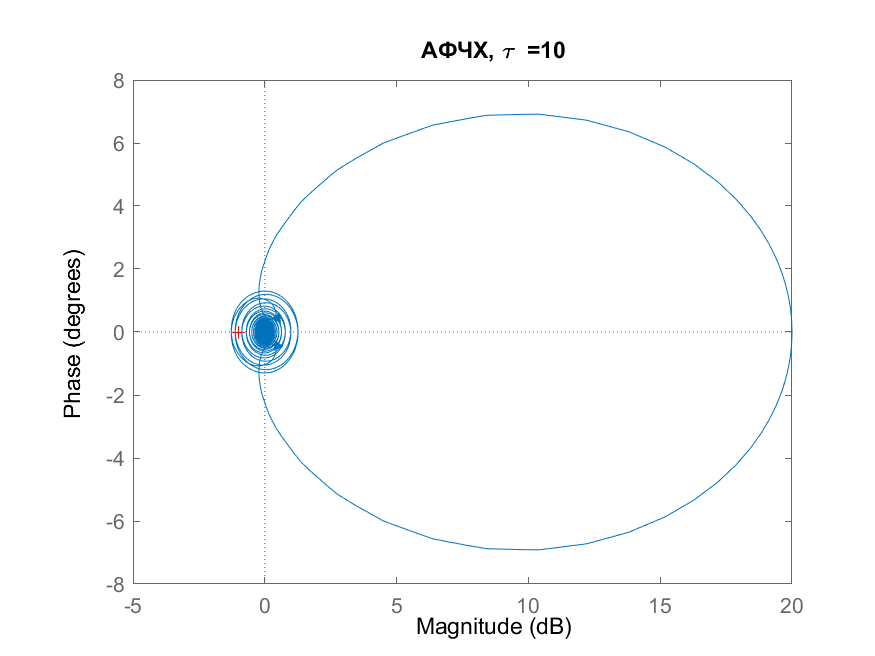
\includegraphics[width=0.7\textwidth]{nyquist_task310_object2.png}
    \caption{Годограф Найквиста для разомкнутой системы, $\tau=10$}
\end{figure}
По полученным графикам пока рано говорить об устойчивости в зависимости от задержки, потому что, например, примерно до $\tau< 0.3$ мы не получаем обороты, которые могут убрать нам неустойчивые полюса, а могут и прибавить, зависит от направления оборотов.
После же, при $\tau > 0.3$ пока рано о чём-либо заявлять, количество и направления трудно установить, поэтому лучше рассмотреть логарифмический критерий Найквиста и аналитически установить диапазон для $\tau$\dots

\newpage
\subsection{Частотные характеристики}
Попробуем найти критическое значение $\tau$. 

\begin{figure}[ht]
    \centering
    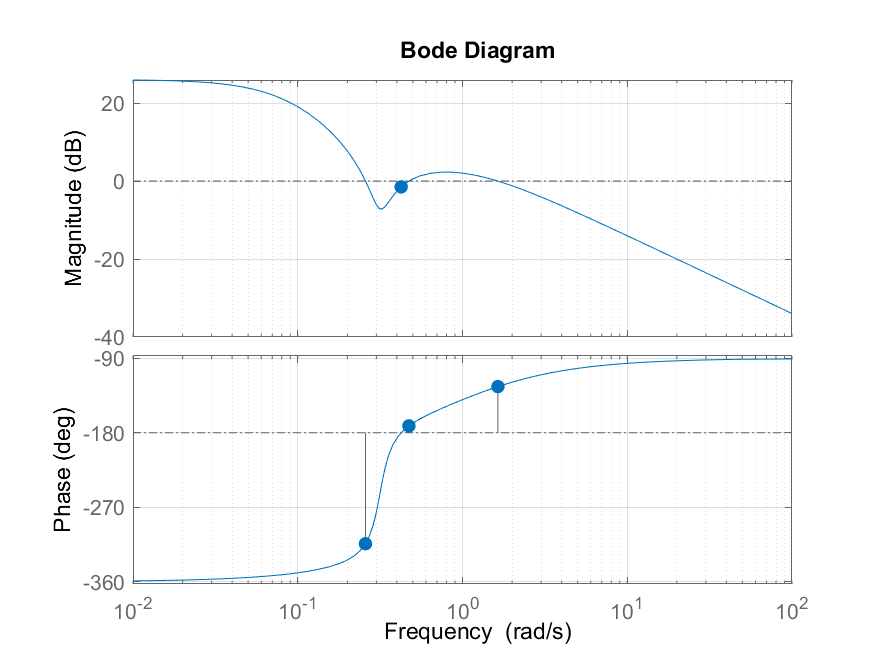
\includegraphics[width=0.7\textwidth]{log_nyquist_task3_object2.png}
    \caption{ЛАФЧХ, $\tau=5.0$}
\end{figure}

Однако всё же с помощью функции \textit{allmargin}  мы можем получить критическое допустимое время запаздывания и запас по фазе для этих точек:


$$
\begin{aligned}
    \tau_{crit1}=15.2, \tab \phi_{13}=-135^\circ, \\   
    \tau_{crit2}=0.3, \tab \phi_{23}=5.5^\circ, \\
    \tau_{crit3}=0.59, \tab \phi_{33}=46^\circ
\end{aligned}
$$

% Как можно заметить их будет три, но при проверке критерия можно заметить:
% нам нужно, чтобы сумма положительных и отриательных переходов через критический отрезок была равна $\frac{r}{2}= 1$. Но при $L(\omega) > 0$ у нас нет переходов, поэтому замкнутая система будет нейстойчивой. У системы не будет запаса устойчивости по фазе.

Как можно заметить, один из кандидатов на запас по фазе у нас отрицательный, поэтому его отбросим и сосредоточимся на двух оставшихся критических точках.

Давайте аналитически посчитаем $\tau_{crit2}, \tau_{crit3}$, которые мы получили от \textit{matlab} до:
$$
\tau_{max} = \frac{\phi_3}{\omega_\phi}
$$, где $\phi_3$ - запас по фазе, $\omega_\phi$ - частота, соответствующая запасу по фазе. Эти два параметра мы можем найти для двух точек, если приблизим график достаточно точно, тогда получим:
$$
\tau_{crit2} = \frac{8.26\pi}{180\cdot 0.4727} \approx 0.304 , \tab \tau_{crit3} = \frac{55.72\pi}{180\cdot 1.6401} \approx 0.59
$$
Получается, что замкнутая система устойчива будет устойчива в диапазоне между двумя критическими значениями, то есть: $\tau \in (0.304; 0.59)$.
Как можно заметить, аналитически посчитанные совпали с ответами от \textit{allmargin}. Проверим это на практике:

\newpage
\subsection{Переходные функции}
\begin{figure}[ht]
    \centering
    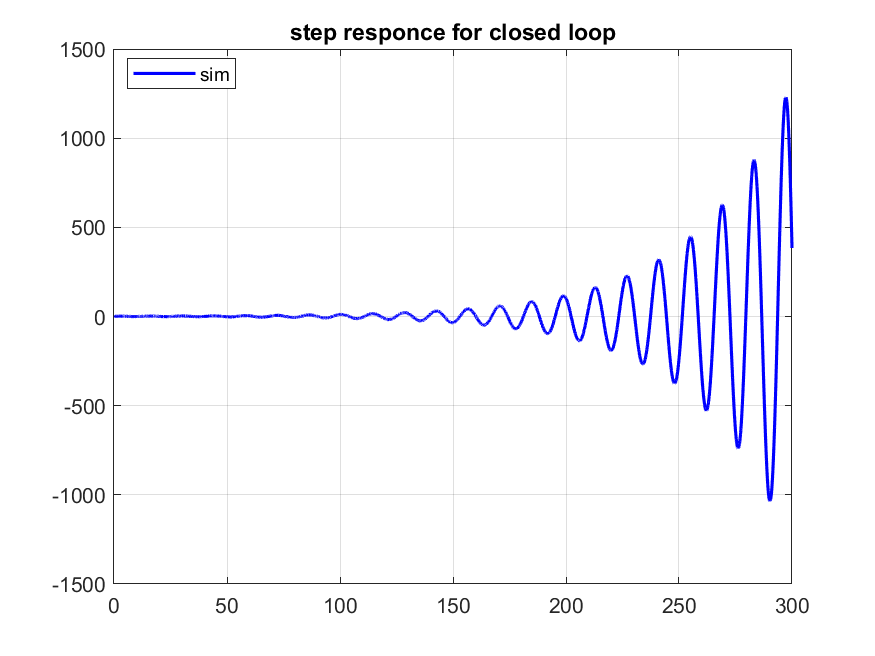
\includegraphics[width=0.7\textwidth]{step_responce31_closed2.png}
    \caption{Переходная функция для замкнутой системы, $\tau=0$}
\end{figure}
\begin{figure}[ht]
    \centering
    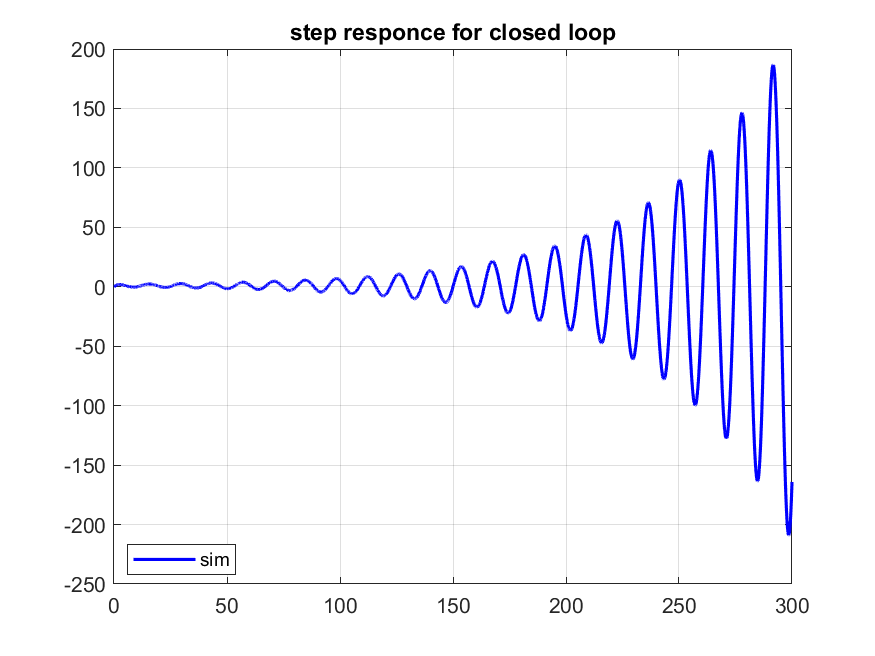
\includegraphics[width=0.7\textwidth]{step_responce32_closed2.png}
    \caption{Переходная функция для замкнутой системы, $\tau=0.1$}
\end{figure}

\newpage
\begin{figure}[ht]
    \centering
    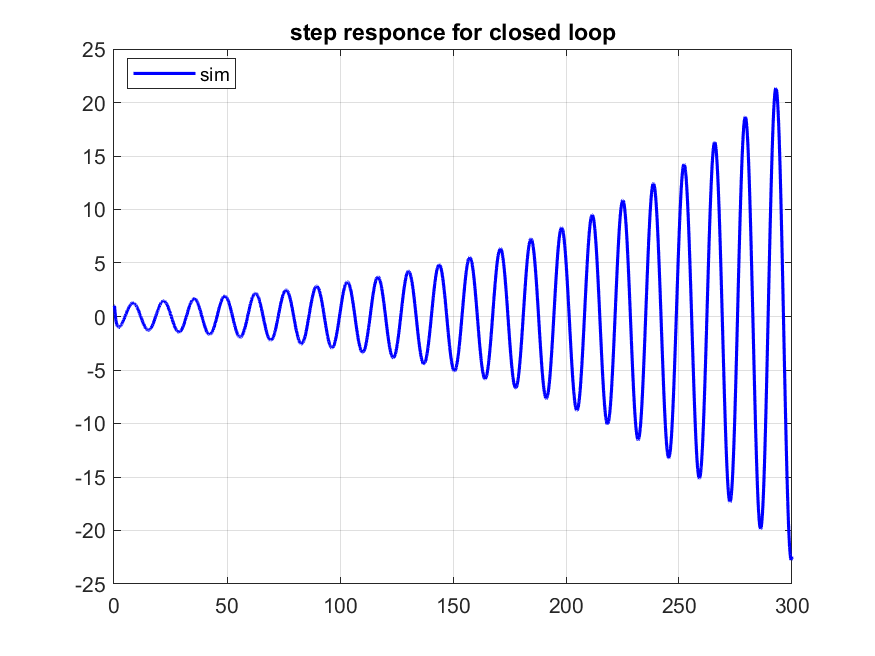
\includegraphics[width=0.7\textwidth]{step_responce33_closed2.png}
    \caption{Переходная функция для замкнутой системы, $\tau=0.2$}
\end{figure}
\begin{figure}[ht]
    \centering
    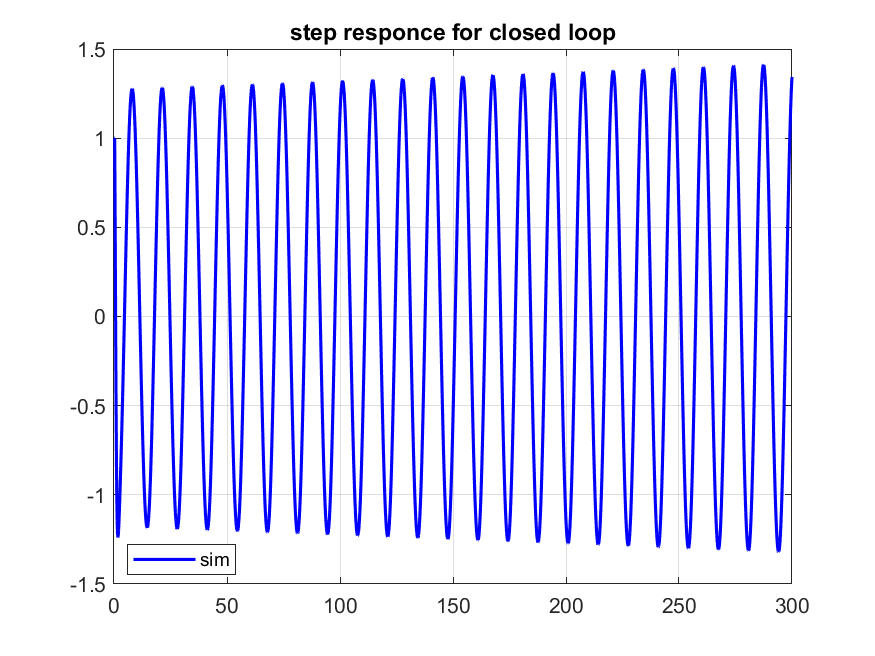
\includegraphics[width=0.7\textwidth]{step_responce34_closed2.png}
    \caption{Переходная функция для замкнутой системы, $\tau=0.3$}
\end{figure}

\newpage
\begin{figure}[ht]
    \centering
    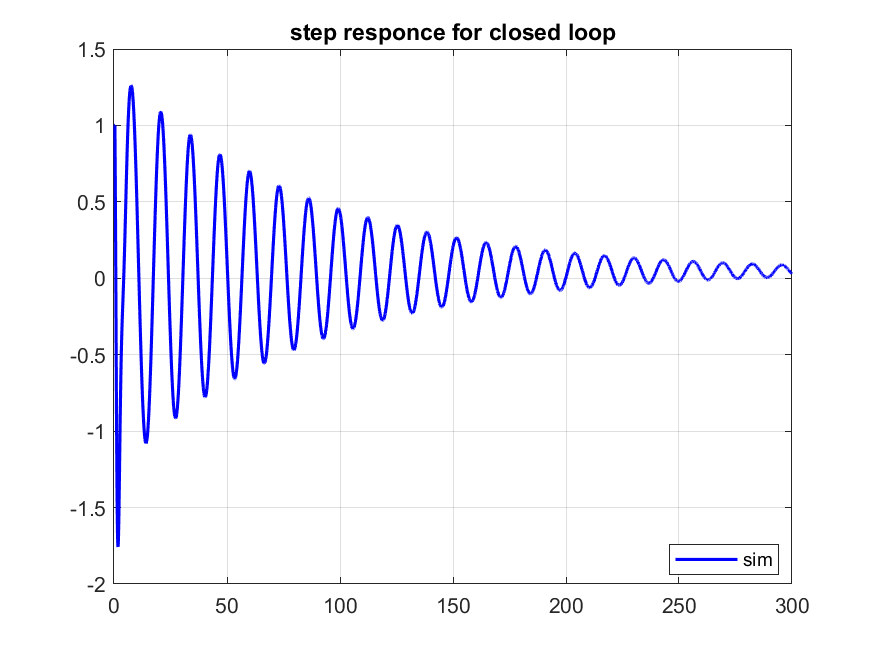
\includegraphics[width=0.7\textwidth]{step_responce35_closed2.png}
    \caption{Переходная функция для замкнутой системы, $\tau=0.4$}
\end{figure}
\begin{figure}[ht]
    \centering
    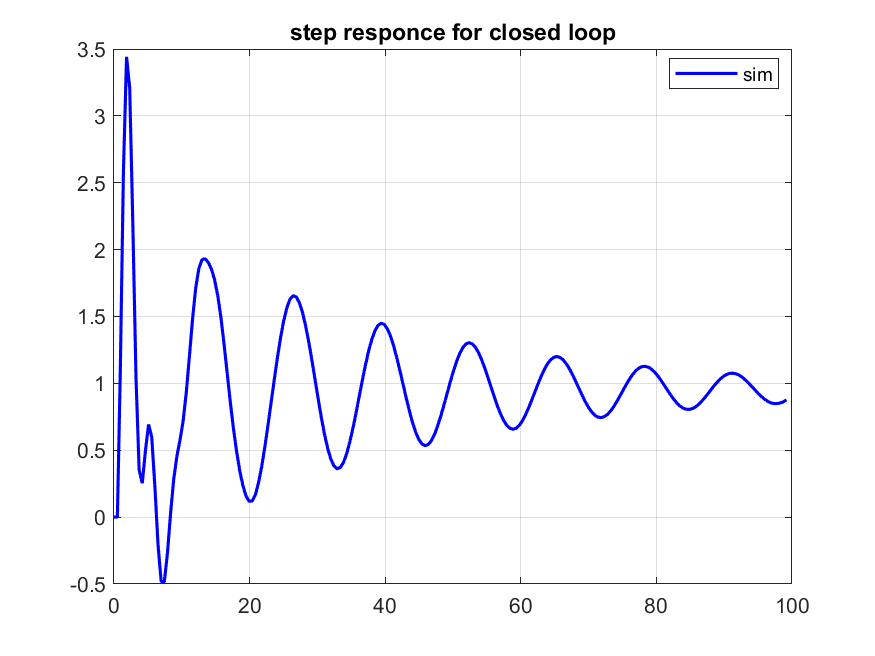
\includegraphics[width=0.7\textwidth]{step_responce36_closed2.png}
    \caption{Переходная функция для замкнутой системы, $\tau=0.5$}
\end{figure}

\newpage
\begin{figure}[ht]
    \centering
    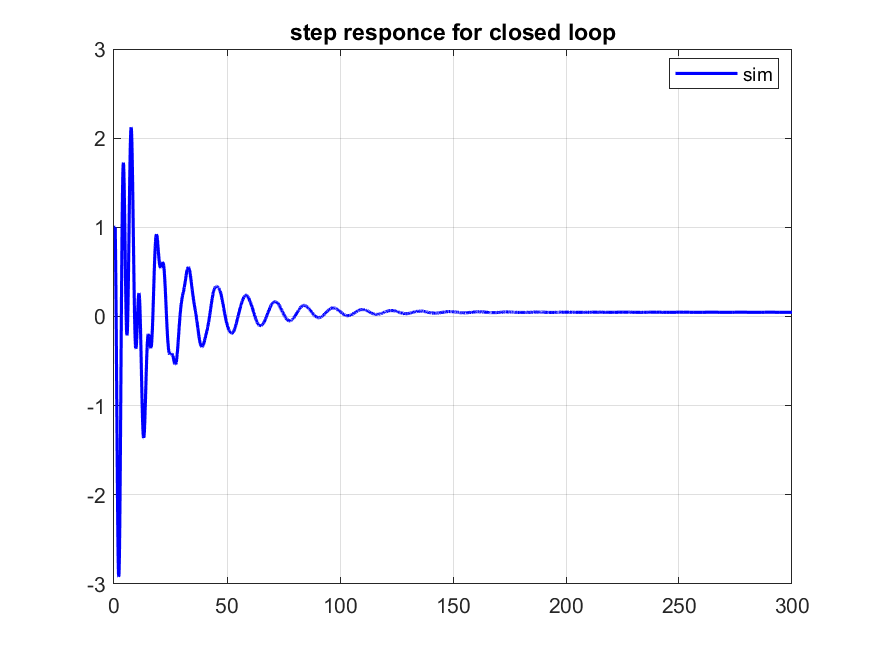
\includegraphics[width=0.7\textwidth]{step_responce37_closed2.png}
    \caption{Переходная функция для замкнутой системы, $\tau=0.55$}
\end{figure}
\begin{figure}[ht]
    \centering
    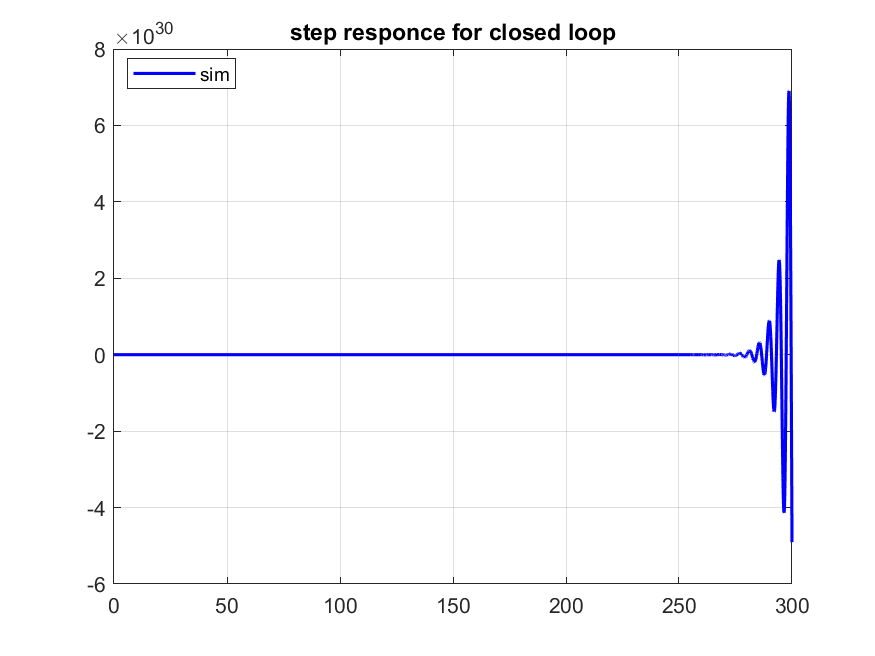
\includegraphics[width=0.7\textwidth]{step_responce38_closed2.png}
    \caption{Переходная функция для замкнутой системы, $\tau=0.7$}
\end{figure}

\newpage
\begin{figure}[ht]
    \centering
    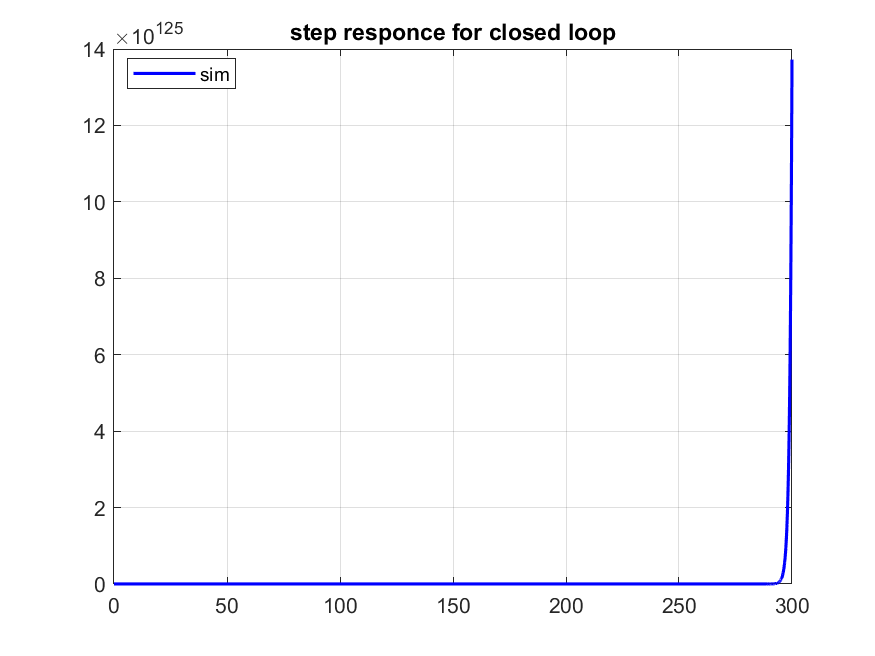
\includegraphics[width=0.7\textwidth]{step_responce39_closed2.png}
    \caption{Переходная функция для замкнутой системы, $\tau=5$}
\end{figure}
\begin{figure}[ht]
    \centering
    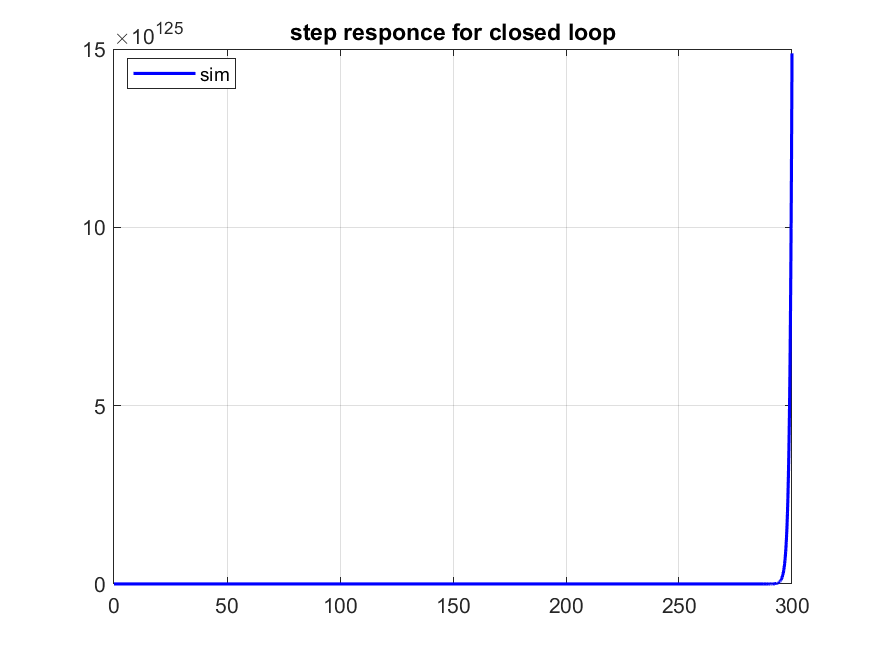
\includegraphics[width=0.7\textwidth]{step_responce310_closed2.png}
    \caption{Переходная функция для замкнутой системы, $\tau=10$}
\end{figure}

По графикам можно заметить, что аналитические выкладки подтвердились - замкнутая система устойчива будет устойчива при $\tau \in (0.304; 0.59)$.

\endinput
\chapter{Пружинка}
\label{ch:chap4}
Параметры системы:
$$
M = 24, \tab k = 112
$$
Даны уравнения пружинного маятника:
$$
F_{ela} = -kx, \tab F = ma = m\ddot{x}
$$
Входом считается $F_{ext}(t)$ - некая внешняя соосно направленная сила, а $x(t)$ - выход. 
Запишем второй закон Ньютона, чтобы объединить уравнения:
$$
    F = F_{ela} + F_{ext} = m\ddot{x}
$$

\section{Передаточная функция}
Перейдем в операторную форму Лапласа:
$$
 -kX + F_{ext} = ms^2X
$$
$$
W(s) = \frac{1}{ms^2 + k}
$$
По отсутствию компоненты $s$ в знаменателе видно, что это - \textit{консервативное звено}, его общий вид:
$$
W(S) = \frac{K}{T^2s^2 + 1}
$$ Тогда в нашем случае $K = \frac{1}{mk} \approx 4\cdot 10^{-4}$ и $T = \sqrt{\frac{1}{k}} \approx 0.09$
\section{Временные  характеристики}
$$
\begin{aligned}
    y_{i.r.}(t) = \mathcal{L}^{-1}\{\frac{K}{T^2s^2 + 1}\} = \mathcal{L}^{-1}\{\frac{K}{T^2(s^2 + \frac{1}{T^2})}\} = \mathcal{L}^{-1}\{\frac{K \frac{1}{T}}{\frac{1}{T}T^2(s^2 + \frac{1}{T^2})}\} = \\
    \frac{K}{T} sin(\frac{1}{T}t)
\end{aligned}
$$
$$
    \begin{aligned}
        y_{s.r.}(t) = \mathcal{L}^{-1}\{\frac{K}{s(T^2s^2 + 1)}\} = \mathcal{L}^{-1}\{\frac{K}{s} - \frac{T^2s}{T^2s^2 + 1}\} = \mathcal{L}^{-1}\{\frac{K}{s} - \frac{Ks}{s^2 + \frac{1}{T^2}}\} = \\
        K - K\cdot cos(\frac{1}{T}t)
    \end{aligned}
$$
\newpage
\begin{figure}[ht]
  \centering
  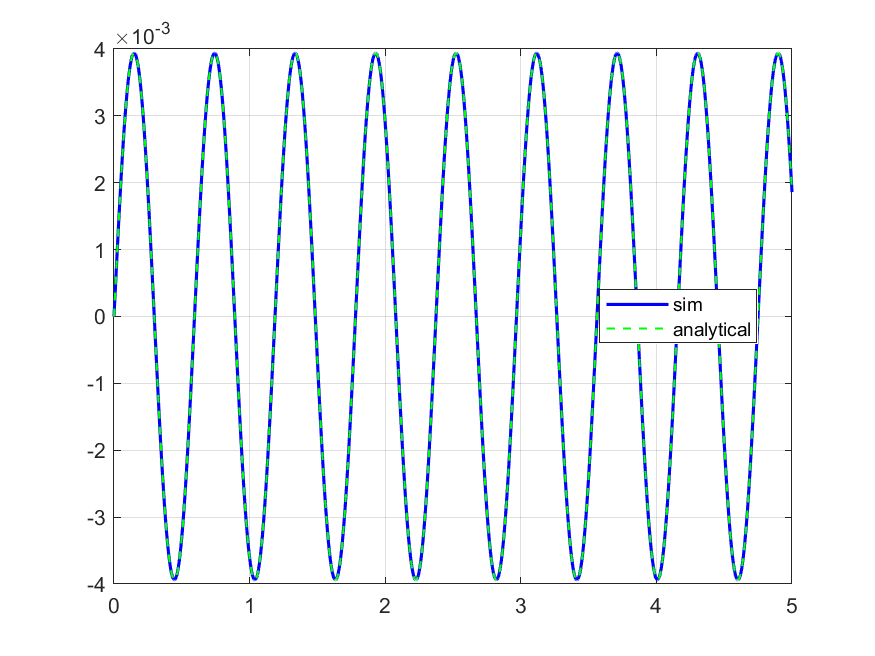
\includegraphics[width=0.8\textwidth]{impulse_responce4.png}
  \caption{Воздействие - \textrm{impulse responce}}
\end{figure}

\begin{figure}[ht]
    \centering
    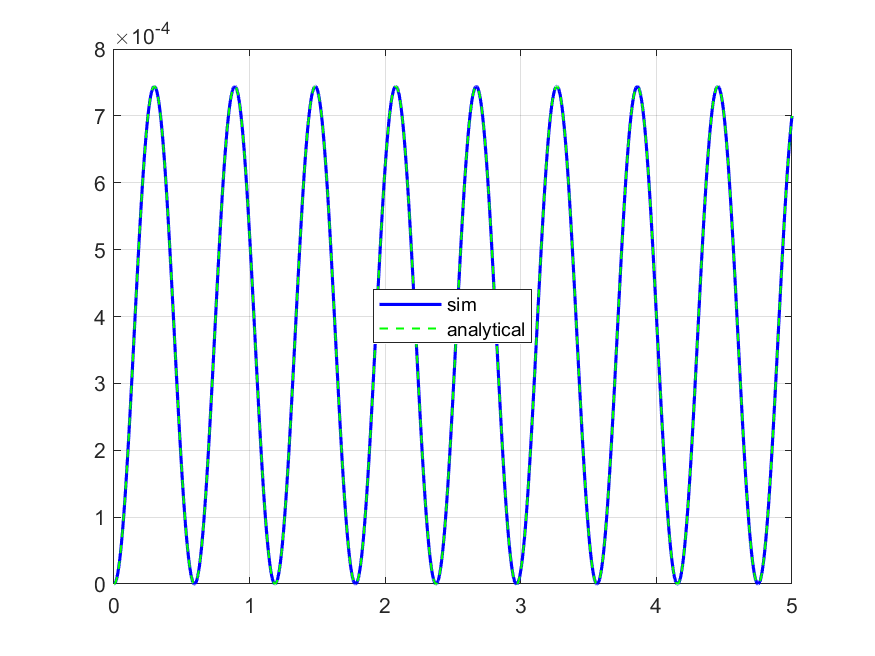
\includegraphics[width=0.8\textwidth]{step_responce4.png}
    \caption{Воздействие - \textrm{step responce}}
  \end{figure}
\newpage
\section{Частотные характеристики}
$$
W(j\omega) =  \frac{K}{T^2(j\omega)^2 + 1} = \frac{K}{1  - T^2\omega^2} + 0
$$
Амплитудно-частотная характеристика:
$$
A(\omega) = \sqrt{P^2 + Q^2} = \sqrt{(\frac{K}{1  - T^2\omega^2})^2 + 0^2} =  \frac{K}{|1  - T^2\omega^2|}
$$
Логарифмическая-Амплитудно-частотная характеристика:
$$
L(\omega) = 20lg(A) = 20lg(K) - 20lg(|1  - T^2\omega^2|)
$$
Фазовая-частотная характеристика:
$$
\phi(\omega) = -atan2(0, \frac{K}{1  - T^2\omega^2})
$$
\newpage
\begin{figure}[ht]
  \centering
  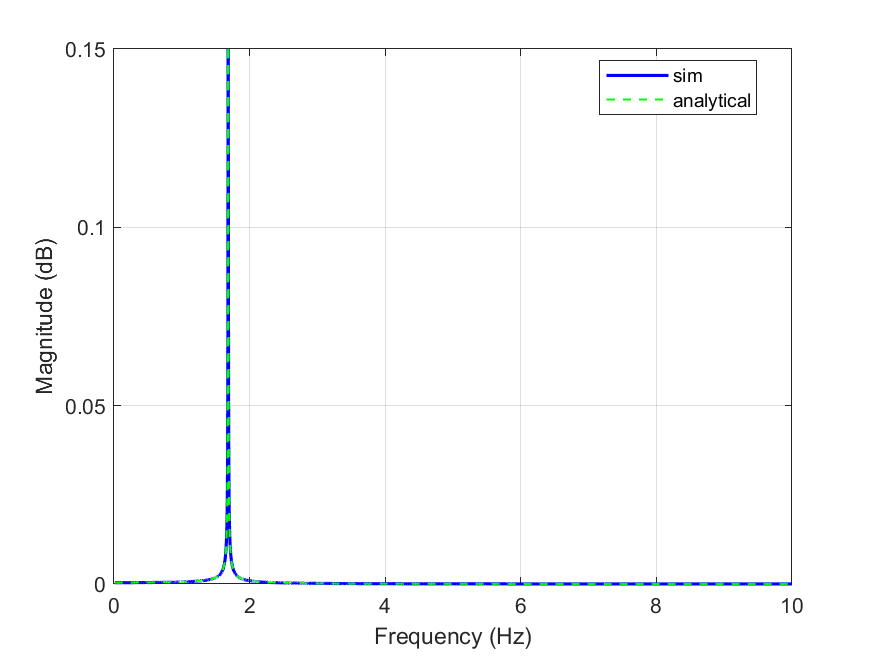
\includegraphics[width=0.8\textwidth]{freq_ampl4.png}
\caption{Сравнение - АЧХ}
\end{figure}

\begin{figure}[ht]
    \centering
    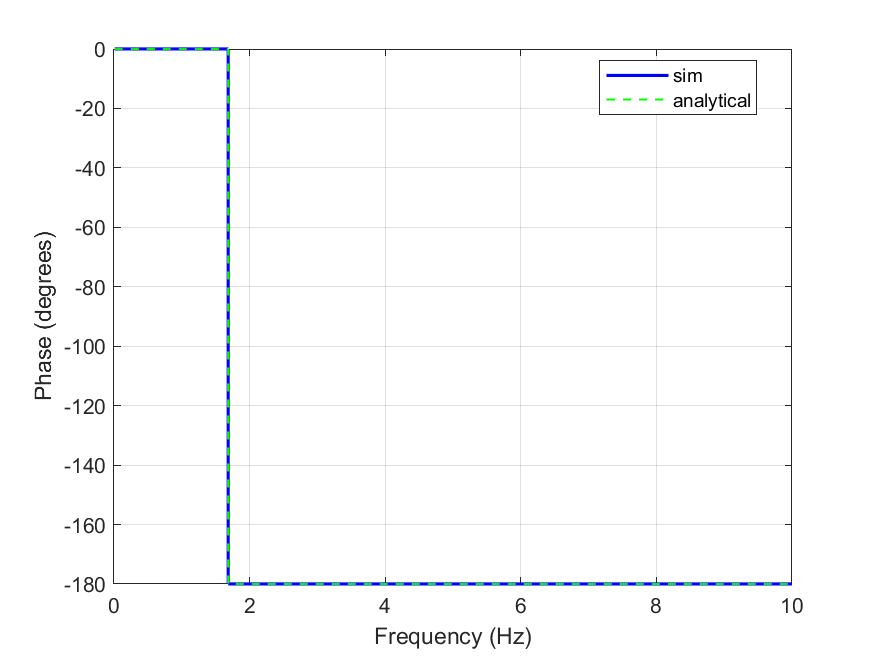
\includegraphics[width=0.8\textwidth]{freq_phase4.png}
  \caption{Сравнение - ФЧХ}
  \end{figure}
\newpage
\begin{figure}[ht]
    \centering
    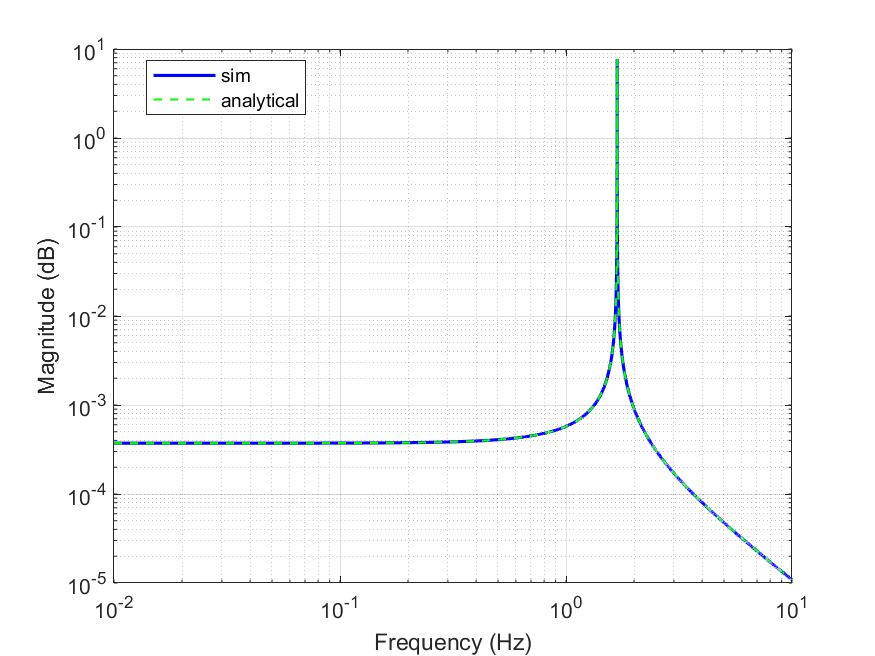
\includegraphics[width=0.8\textwidth]{lfreq_ampl4.png}
  \caption{Сравнение - ЛАЧХ}
  \end{figure}
  
  \begin{figure}[ht]
      \centering
      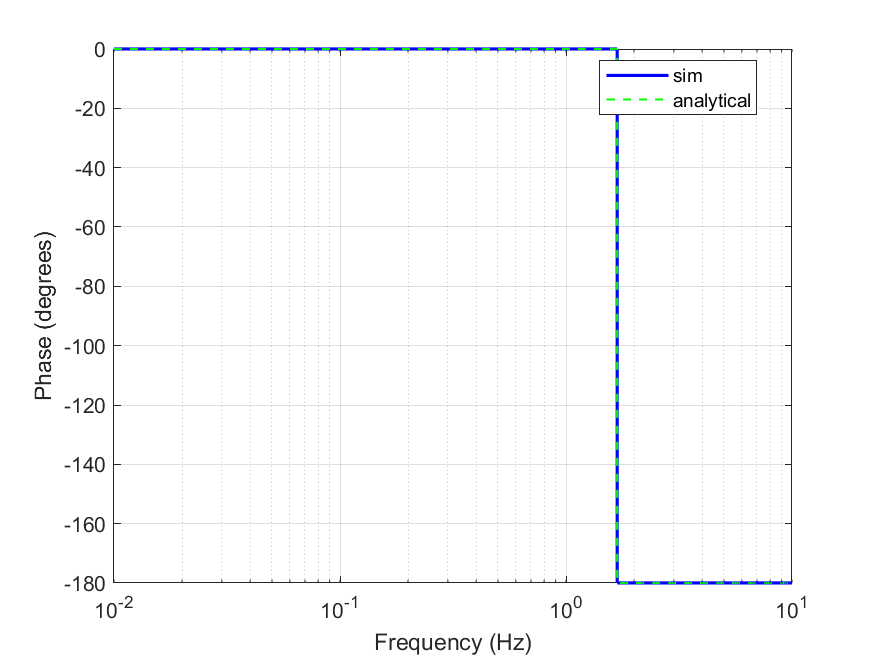
\includegraphics[width=0.8\textwidth]{lfreq_phase4.png}
    \caption{Сравнение - ЛФЧХ}
    \end{figure}

    % \begin{figure}[ht]
    %   \centering
    %   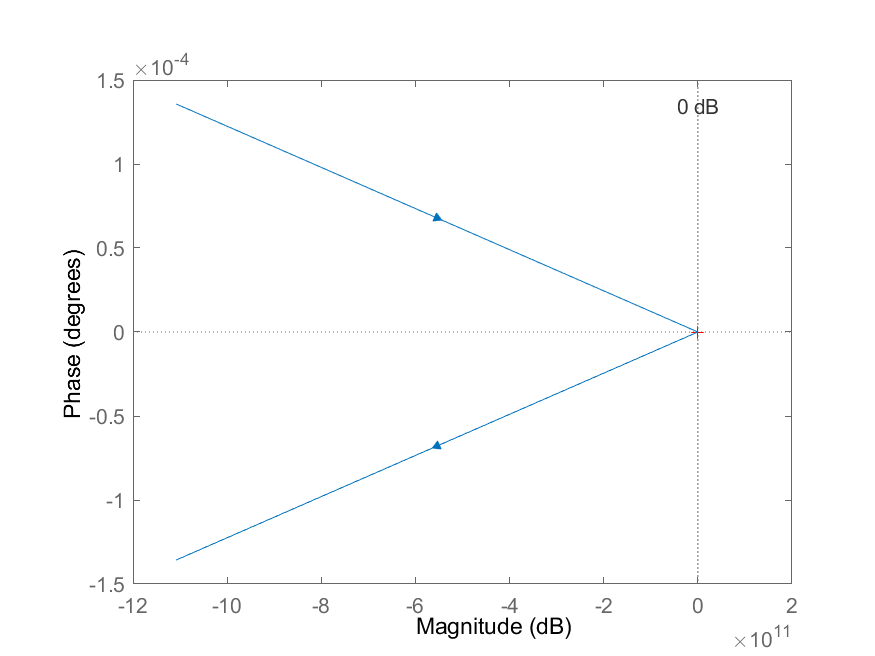
\includegraphics[width=0.8\textwidth]{nyquist4.png}
    % \caption{АФЧХ}
    % \end{figure}
\newpage

\endinput
\chapter{Исследование управляемости по выходу}
\label{ch:chap5}
\section{Условие задачи}

Необходимо рассмотреть систему:
$$
  \begin{cases}
    \dot{x} = Ax + Bu \\
    y = Cx + Du
  \end{cases}
$$ и выполнить следующие шаги:

\begin{itemize}
    \item Найти Жорданову (или диагональную) форму системы.
    \item Определить управляемость и наблюдаемость каждого из собственных чисел и системы в целом.
    \item Найти матрицу управляемости системы по выходу при $D = \mathbf{0}_{2×2}$, определить её
    ранг, сделать вывод об управляемости системы по выходу.
    \item Проанализировав полученные результаты, попытаться сделать выводы о причинах 
    управляемости или неуправляемости системы по выходу.
    \item Предложить такую матрицу cвязи $D$, которая могла бы обеспечить 
    полную управляемость по выходу.
\end{itemize}

\section{Решение задачи}

Параметры для объекта:
$$
  A = \begin{bmatrix}
  3 & -6 & 4 \\
  4 & -5 & 4 \\
  -4 & 4 & -5 
  \end{bmatrix} \tab
  B = \begin{bmatrix}
    -1 \\ 3 \\ 1 
  \end{bmatrix} \tab
  C = \begin{bmatrix}
    0 & -4 & -3 \\
    0 & -8 & -6
  \end{bmatrix}
$$

\subsection{Исследование управляемости и наблюдаемости системы}


Найдём Жорданову форму системы, в общем виде она выглядит следующим образом:
$$
    \begin{cases}
      \dot{\hat{x}} = P^{-1}\boldsymbol{A}P \hat{x} + P^{-1}\boldsymbol{B} u \\
      y = \boldsymbol{C}P\hat{x} + Du
    \end{cases}
$$
В нашем случае жорданова клетка и входное/выходное воздействие таково:
$$
    \mathbf{A} = \begin{bmatrix}
        -1 & 0 & 0 \\
        0 & -3 & -2 \\
        0 & 2 & -3 
        \end{bmatrix} \tab 
    P^{-1}B = B^* = \begin{bmatrix}
        4 \\ -1.5+1.5i \\ -1.5-1.5i
        \end{bmatrix}
$$
$$
    CP= \begin{bmatrix}
        -3 & 1 & 1 \\
        -6 & 2 & 2 
        \end{bmatrix}
$$
Как можно заметить, три собственных числа соответствуют различным жордановым клеткам, и для каждой из них строка матрицы входных/выходных воздействий не равна нулю.
Значит эти три собственных числа управляемы и наблюдаемы, и как следствие - вся система полностью управляема по состоянию и наблюдаема.





Найдем матрицу управляемости системы по выходу при $D = \mathbf{0}_{2×2}$ :

$$
    U_{out} = \begin{bmatrix}
      CU & D
    \end{bmatrix} =  \begin{bmatrix}
      -15 & 27 & -63 & 0 & 0 \\
      -30 & 54 & -126 & 0 & 0 
    \end{bmatrix}
$$
Нетрудно заметить, что\dots
$$
  rank(U_{out}) = 1
$$
Ранг матрицы управляемости по выходу не равен размерности выхода, в таком случае наша система не управляема по выходу.

Это произошло из-за того, что матрица матрица наблюдения $C$ содержит в себе два линейнозависимых вектора-строки, которые снижают ранг до 1.
Также из-за этого мы теряем информацию по выходу $y(t)$, потому что обе компоненты вектора станет созависимыми и мы не сможем обеспечить все возможные выходы у системы.

Чтобы исправить это и сделать систему управляемой по выходу, необходимо подобрать такую матрицу $D$, которая сделает ранг $U_{out}=2$. 
Например: 
$$
    D = \begin{bmatrix}
        1 & 0 \\
        0 & 1
    \end{bmatrix}
$$
Тогда матрица управляемости по выходу будет равна:
$$
    U^*_{out} = \begin{bmatrix}
      CU & D
    \end{bmatrix} =  \begin{bmatrix}
      -15 & 27 & -63 & 1 & 0 \\
      -30 & 54 & -126 & 0 & 1 
    \end{bmatrix}
$$
и её ранг уже будет равен 2.

\subsection{Вывод}

В этом задании мы рассмтрели полная линейную систему. Мы нашли жорданову форму систему, по которой мы исследовали управляемость по состоянию и наблюдаемость, 
вышло, что система управляема по состоянию и наблюдаема. Однако при этом нулевая матрица связи $D_{2×2}$ не делала эту систему упроавляемой по выходу, но
мы нашли подходящую.
\endinput
\chapter{Общие выводы}
\label{ch:chap6}

В ходе выполнения лабораторной работы был рассмотрен синтез модального регулятора и наблюдателя (полный/пониженного порядка) по отдельности, а также вместе(стандартный линейный регулятор по выходу). 
Синтез осуществлялся при помощи метода уравнения Сильвестра, синтезированные компоненты системы проверялись при помощи компьютерного моделирования, наблюдатель успешно сходился к истинной системе, 
а регулятор успешно приводил в положение равновесия.

Использовал связку \textit{Live-script + Matlab}, все исходные материалы, использованные в работе можно найти  в \href{https://github.com/GreedlyCore/control_theory_course}{репозитории}. 
\endinput

% \printbibliography[title=Список использованных источников] % Автособираемый список литературы

\end{document}